\chapter{Experimental Results and Analysis}
\label{ch:results}
\label{ch:analysis}

This chapter presents the quantitative results of the experiments carried out in this thesis, together with their interpretation, topic by topic. It opens by presenting the benchmarks used throughout the thesis and formally defining the metrics computed over them, both the average accuracy and forgetting scores and the complementary confidence and calibration metrics. From there, the covariance estimators and mixture-of-Gaussian variants results are presented, then how well-calibrated their predictions actually are, then how the system behaves as more classes are added over time, and how separable classes are from one another in the embedding space. It then looks at the feature space itself---its sensitivity to the choice of backbone, its spectral structure, and how well it satisfies the Gaussianity assumption the whole framework rests on---and closes by weighing the computational cost of the framework before summarising the practical conclusions that follow from all of this evidence taken together.

Before going further, it is worth fixing the short names used repeatedly in the tables and discussion below. \textbf{Diag-Cov} and \textbf{Full-Cov} are the two basic covariance parameterisations introduced in Section~\ref{sec:covariance_estimation}: a diagonal covariance matrix, which treats feature dimensions as independent of one another, and a full covariance matrix, which also captures the correlations between them. \textbf{Hybrid-Cov} is the intermediate estimator that keeps the full covariance structure for the Mahalanobis, shape-related term of the discriminant, while using only its diagonal for the log-determinant, volume-related term. \textbf{OAS} and \textbf{LW-I}/\textbf{LW-D} are the two shrinkage-based estimators introduced in the same section: Oracle Approximating Shrinkage, and Ledoit--Wolf shrinkage toward an Identity or a Diagonal target, respectively. The prefix \textbf{Shared-} (as in Shared-Diag-Cov or Shared-Full-Cov) means that the corresponding covariance is estimated once, globally, and reused across every class, rather than independently per class. Finally, \textbf{MOG2} and \textbf{MOG4} denote mixture-of-Gaussian variants with exactly two, or with up to four, components per class, respectively; the trailing letter---\textbf{D}, \textbf{F}, or \textbf{H}---again indicates whether each individual component uses a diagonal, full, or hybrid covariance, and \textbf{MOG4-Shared} combines the multi-component MOG4 formulation with a single, globally shared full-covariance matrix.

For every benchmark we report the average accuracy after the last task, $A_{T}$, and the forgetting score $F_{T}$, both formally defined below. Whenever possible we report mean and variance over three independent runs (different task-order seeds). Since the proposed Gaussian classifiers maintain only sufficient statistics $(\boldsymbol{\mu}_c, \boldsymbol{\Sigma}_c)$ and do not involve parameter optimisation during incremental updates, the resulting classifier is independent of the specific class-presentation order; this explains the $\pm 0.00$ standard deviation reported for our methods throughout. State-of-the-art prompt-based competitors are reproduced from the published values reported in their respective papers. Methods proposed in this thesis are highlighted in grey. The best result per column is shown in bold.

\section{Image Datasets and Benchmarks}
\label{sec:an:datasets}

Before reporting any empirical result, this section presents the four benchmarks evaluated throughout this thesis. We first introduce the underlying image datasets and what makes each one relevant to this work, and then explain how each one is turned into a class-incremental stream.

\subsection{Source Datasets}
\label{sec:an:source_datasets}

Three source datasets are used to build the benchmarks of this thesis, chosen so that, together, they vary in image resolution, visual style, and category granularity. \textbf{CIFAR-100} \cite{cifar100} contains 60,000 low-resolution ($32\times32$) natural images, organised into 100 ``fine'' classes grouped under 20 broader ``coarse'' categories. \textbf{Caltech-256} \cite{caltech256} contains 30,607 higher-resolution images spread across 256 categories, with more images per class and more visual diversity than CIFAR-100; in this thesis, we use its first 250 categories, for reasons explained below. \textbf{ImageNet-R} \cite{imagenetR} takes 200 of the classes from the original ImageNet \cite{imagenet} and replaces their photographs with 30,000 non-photographic renditions instead, such as paintings, cartoons, and sketches, which makes it well suited for testing robustness to this kind of stylistic domain shift. A fourth, much larger dataset, \textbf{ImageNet-21k} \cite{imagenet21k}, is not itself turned into a benchmark in this section, but is used elsewhere in this thesis as pre-training data, both for the backbones compared in Section~\ref{sec:backbone_results} and for the fixed projection matrix used in the PCA probe of Section~\ref{sec:spectral_analysis}.

\subsection{Continual Learning Splits and Protocol}
\label{sec:an:cl_splits}

Each of the three source datasets above is turned into a class-incremental benchmark by splitting its classes into a fixed sequence of disjoint tasks, following the standard protocol described in Chapter~\ref{methodology}: the model sees one task at a time, and average accuracy and forgetting, formally defined in Section~\ref{sec:an:metrics}, are computed over the classes seen so far. A fourth benchmark then combines all three streams into a single, longer one. Concretely:

\begin{itemize}
	\item \textbf{Split CIFAR-100} divides the 100 classes into 10 disjoint tasks of 10 classes each.

	\item \textbf{Split ImageNet-R} divides its 200 classes, randomly, into 10 tasks of 20 classes each; because its images are stylistic renditions rather than plain photographs, this split also introduces a deliberate domain-shift challenge on top of the usual class-incremental one.

	\item \textbf{Split Caltech-256} keeps only the first 250 of the original 256 categories, so that they divide evenly into 10 balanced tasks of 25 classes each (the remaining six categories are simply discarded). The resulting stream has around 28\,100 images and an average of $\overline{n_c}\!\approx\!112$ training samples per class, the smallest per-class budget of the three datasets, which makes it the one that puts the most pressure on the high-dimensional covariance estimators of Section~\ref{sec:covariance_estimation}.

	\item \textbf{Split Joint} concatenates the 30 tasks of the three benchmarks above into a single, heterogeneous, 30-task stream, presented to the model in a randomised order. This forces the classifier to move between natural, artistic, and high-resolution images within the same run, and is meant to stress-test the framework over a much longer and more varied stream than any of the three individual benchmarks alone.
\end{itemize}

\subsection{Benchmark Properties Summary}
\label{sec:an:benchmark_summary}

The four resulting benchmarks span a wide spectrum of statistical difficulty for a Gaussian classifier. Their salient properties are summarised in Table~\ref{tab:dataset_summary}.

\begin{table}[htbp]
	\centering
	\caption{Statistical characterisation of the four benchmarks. $\overline{n_c}$ denotes the average sample budget per class.}
	\label{tab:dataset_summary}
	\scriptsize
	\setlength{\tabcolsep}{4pt}
	\begin{tabular}{lcccccc}
		\toprule
		\textbf{Benchmark} & \textbf{\# Classes} & \textbf{\# Tasks} & \textbf{Image source} & $\overline{n_c}$\\
		\midrule
		Split CIFAR-100   & 100 & 10 & Natural, low-resolution ($32{\times}32$)   & $500$    \\
		Split ImageNet-R  & 200 & 10 & Renditions: art, sketch, cartoon          & $150$     \\
		Split Caltech-256 & 250 & 10 & Natural, high-resolution, variable scale  & $112$  \\
		Split Joint       & 550 & 30 & Heterogeneous concatenation of the above  & mixed    \\
		\bottomrule
	\end{tabular}
\end{table}

The three primary datasets differ along two largely orthogonal axes: visual complexity (which determines how heavy-tailed the embedding coordinates are) and sample budget (which determines how reliably the per-class covariance can be estimated). CIFAR-100 occupies the favourable corner of both axes, ImageNet-R adds a deliberate input-distribution shift, and Caltech-256 combines heavy tails with a small per-class budget. The Joint benchmark inherits the worst feature of each of the three constituent datasets and is therefore the most informative regime for separating method behaviour. With the benchmarks now fully characterised, we turn to the evaluation metrics computed over them.

\section{Evaluation Metrics: Average Accuracy and Forgetting}
\label{sec:an:metrics}

 As is common in the continual learning literature \cite{wang2022learning}, we quantify performance using two standard metrics derived from the test accuracy scores obtained after each task: the average accuracy and the average forgetting.

On the one hand, \textbf{Average Accuracy ($A_t$)}, presented on equation \eqref{eq_AA}, measures overall performance after task $t$. It is the mean test accuracy across all tasks learned up to that point.

\begin{equation}
	A_t = \frac{1}{t} \sum_{\tau=1}^{t} S_{t,\tau}
	\label{eq_AA}
\end{equation}

On the other hand, \textbf{Forgetting ($F_{t}$)}, presented on equation \eqref{eq_AF}, quantifies how much the model has forgotten earlier tasks. It computes, for each past task, how much accuracy has dropped compared to its best historical score, and averages those drops.

\begin{equation}
	F_t = \frac{1}{t-1} \sum_{\tau=1}^{t-1} \left( \max_{k \le t-1} S_{k,\tau} - S_{t,\tau} \right)
	\label{eq_AF}
\end{equation}

Regarding forgetting, the proposed framework does not exhibit forgetting in the conventional sense, as previously learned class statistics are never modified when new classes are introduced. The measured forgetting values therefore primarily reflect the increased classification difficulty as the number of competing classes grows, rather than degradation of previously learned representations.

\section{Confidence and Calibration Metrics}
\label{sec:an:calibration_metrics_def}

Accuracy and forgetting measure whether the model's predictions are correct, but they say nothing about whether the model's own confidence in those predictions can be trusted---a distinction that matters in particular for Class-Incremental Learning, where a classifier can look accurate while still being systematically over- or under-confident. To capture this, we introduce five complementary metrics that jointly characterise the probabilistic behaviour of the classifier: the Expected Calibration Error (ECE) measures the global alignment between confidence and accuracy; the Confidence on Errors (CoE) quantifies how dangerously overconfident the model is when it fails; Total Confidence (TC) and Probability Margin (PM) both capture the decisiveness of the posterior distribution from two complementary angles; and the Average Predictive Entropy ($H$) measures the spread of probability mass across all classes. These definitions are used directly in Section~\ref{sec:calibration_results_section}, where the resulting values are reported and interpreted.

\subsection{Expected Calibration Error (ECE)}
This metric quantifies the mismatch between predictive confidence and empirical accuracy. We partition the predictions into $M$ equally spaced bins based on their confidence scores. The ECE is defined as the weighted average of the absolute difference between the accuracy and confidence of each bin:

\begin{equation}
	ECE_t = \sum_{m=1}^{M} \frac{|B_m|}{N} \left| acc(B_m) - conf(B_m) \right|\label{eq_ECE}
\end{equation}

where $N$ is the total number of samples, $B_m$ is the set of indices of samples whose prediction confidence falls into the $m$-th interval, and $acc(B_m)$ and $conf(B_m)$ represent the mean accuracy and mean confidence within that bin, respectively.

\subsection{Confidence on Errors (CoE)}
To specifically analyze the model's behavior when it fails, we measure the average confidence assigned to the winning (but incorrect) class. High CoE indicates a model that is ``dangerously wrong'', which matters in safety-oriented applications. It is computed for a task $t$ as:

\begin{equation}
	CoE_t = \frac{1}{|\mathcal{E}_t|} \sum_{i \in \mathcal{E}_t} \max(\hat{p}_i)
\end{equation}

where $\mathcal{E}_t$ is the set of misclassified samples and $\hat{p}_i$ is the predicted probability distribution for sample $i$.

\subsection{Total Confidence (TC)}

Total Confidence measures how certain the model is on average about its top-1 prediction, regardless of whether that prediction is correct:

\begin{equation}
	TC_t = \frac{1}{N} \sum_{i=1}^{N} \max_{c} \, p_{i,c}
\end{equation}

A value of $TC=1$ means the model assigns all probability mass to a single class for every sample---it is always maximally decisive. A value close to $1/C$ would indicate near-uniform posteriors. TC is a measure of \emph{decisiveness}, not correctness: a well-calibrated model should have $TC \approx A_T$ (confident when right, uncertain when wrong), whereas a badly overconfident model can reach $TC \approx 1$ even at low accuracy.

\subsection{Probability Margin (PM)}

The Probability Margin is the natural, non-logarithmic measure of how decisively the model separates its top-1 prediction from its second-best alternative:

\begin{equation}
	PM_t = \frac{1}{N} \sum_{i=1}^{N} \Bigl( p_{i,(1)} - p_{i,(2)} \Bigr)
\end{equation}

where $p_{i,(1)} \ge p_{i,(2)}$ are the two highest posterior probabilities for sample $i$. A margin near $1$ means the model almost entirely ignores its second candidate; a margin near $0$ means the model is nearly tied between its top-two guesses and one should treat the prediction with caution. PM is bounded in $[0,1]$ and directly interpretable: a value of $0.7$ means the winning class is, on average, assigned $70\%$ more probability than the runner-up.

\subsection{Average Predictive Entropy ($H$)}
We utilize Shannon entropy to measure the uncertainty of the model's predictions. A higher entropy suggests that the model is distributing its probability mass across multiple classes, indicating lower certainty. For task $t$, the average entropy is calculated as:

\begin{equation}
	H_t = \frac{1}{N} \sum_{i=1}^{N} \left( - \sum_{c=1}^{C} p_{i,c} \log(p_{i,c}) \right)
\end{equation}

where $p_{i,c}$ is the probability assigned to class $c$ for sample $i$.

\subsection*{Summary of calibration and uncertainty metrics}

Table~\ref{tab:metrics_summary} collects all six metrics (accuracy and the five calibration/uncertainty indicators), their range, the direction of improvement, and the key question each one answers. Together they provide a multi-dimensional view of the model's reliability throughout continual learning: accuracy tells us \emph{how often} the model is right; ECE tells us \emph{how well-calibrated} its probabilities are; CoE tells us \emph{how dangerous} its mistakes are; TC tells us \emph{how decisive} it is overall; PM tells us \emph{how clearly} it separates its top-two candidates; and entropy tells us \emph{how spread} its uncertainty is across all classes.

\begin{table}[htb]
	\centering
	\caption{Summary of the probabilistic calibration and uncertainty metrics used in this work. ``Better'' indicates the direction of the preferred value; ``context'' means both high and low values are informative depending on whether predictions are correct.}
	\label{tab:metrics_summary}
	\scriptsize
	\setlength{\tabcolsep}{5pt}
	\renewcommand{\arraystretch}{1.25}
	\begin{tabular}{llcll}
		\toprule
		\textbf{Metric} & \textbf{Symbol} & \textbf{Range} & \textbf{Better} & \textbf{Key question} \\
		\midrule
		Accuracy                    & $A_T$  & $[0,1]$         & $\uparrow$   & What fraction of predictions are correct? \\
		Expected Calibration Error  & ECE    & $[0,1]$         & $\downarrow$ & How well does confidence match actual accuracy? \\
		Confidence on Errors        & CoE    & $[0,1]$         & $\downarrow$ & How confident is the model when it is \emph{wrong}? \\
		Total Confidence            & TC     & $[0,1]$         & context      & How decisive is the model on its top-1 choice? \\
		Probability Margin          & PM     & $[0,1]$         & context      & How much more likely is top-1 than top-2? \\
		Predictive Entropy          & $H$    & $[0, \log C]$   & $\downarrow$ & How spread is probability mass over all $C$ classes? \\
		\bottomrule
	\end{tabular}
\end{table}

With accuracy, forgetting, and the confidence and calibration metrics now all formally established, we turn to the empirical results themselves, beginning with the covariance estimators and mixture-of-Gaussian variants.

\section{Covariance Estimator and Mixture-of-Gaussian Results}

\label{sec:covariance_results}
Table~\ref{tab:combined_benchmarks} reports the average accuracy and the forgetting score for every covariance estimator (diagonal, full, hybrid, Ledoit--Wolf identity/diagonal target~\cite{Ledoit2004}, OAS~\cite{Chen2010}) and for the mixture-of-Gaussian variants MOG-$k$ with $k\in\{2,4\}$ components and three sub-variants (\textit{D}, \textit{F}, \textit{H} for diagonal, full and hybrid covariance respectively). 
To ensure statistical robustness, all proposed configurations are evaluated across three independent experimental runs using distinct randomized task-presentation seeds, with performance reported as the sample mean alongside its corresponding standard deviation. For the state-of-the-art baselines, these variance metrics are included when available from their original literature sources.
The table is organised in three blocks: prompt-based state-of-the-art baselines reproduced from the literature (L2P, DualPrompt, APT); analytic, feature-based baselines (SimpleCIL, FeCAM, RanPAC); and, at the bottom, the proposed Gaussian estimators. Table~\ref{tab:split_joint} reports the same family on the 30-task Joint stream.

\begin{table}[htb]
	\centering
	\caption{Continual-learning performance on the three 10-task benchmarks. $A_{10}$ and $F_{10}$ are reported in percentage points.}
	\label{tab:combined_benchmarks}
	\scriptsize
	\begin{tabularx}{\textwidth}{lXXXXXX}
		\toprule
		\textbf{Method} & \multicolumn{2}{c}{\textbf{Split CIFAR-100}} & \multicolumn{2}{c}{\textbf{Split ImageNet-R}} & \multicolumn{2}{c}{\textbf{Split Caltech-256}} \\
		\cmidrule(lr){2-3} \cmidrule(lr){4-5} \cmidrule(lr){6-7}
		& \multicolumn{1}{c}{$A_{10} (\uparrow)$} & \multicolumn{1}{c}{$F_{10} (\downarrow)$} & \multicolumn{1}{c}{$A_{10} (\uparrow)$} & \multicolumn{1}{c}{$F_{10} (\downarrow)$} & \multicolumn{1}{c}{$A_{10} (\uparrow)$} & \multicolumn{1}{c}{$F_{10} (\downarrow)$} \\
		\midrule
		L2P             & $83.86 \pm 1.17$ & $7.35 \pm 0.39$ & $61.57 \pm 0.40$ & $9.73 \pm 0.42$ & $92.11 \pm 0.32$ & $2.94 \pm 0.26$ \\
		DualPrompt      & $86.51 \pm 0.49$ & $5.16 \pm 0.20$ & $68.13 \pm 0.52$ & $4.68 \pm 0.18$ & $92.50 \pm 0.16$ & $2.50 \pm 0.16$ \\
		DualPrompt-PGP  & $86.92 \pm 0.05$ & $5.35 \pm 0.19$ & $69.34 \pm 0.05$ & $4.53 \pm 0.04$ & \multicolumn{1}{c}{---} & \multicolumn{1}{c}{---} \\
		CODA-Prompt     & $87.00 \pm 0.38$ & $4.78 \pm 0.24$ & $74.24 \pm 0.56$ & $4.92 \pm 0.21$ & \multicolumn{1}{c}{---} & \multicolumn{1}{c}{---} \\
		CPrompt         & $87.83 \pm 0.37$ & $4.88 \pm 0.79$ & $76.71 \pm 0.61$ & $4.66 \pm 0.93$ & \multicolumn{1}{c}{---} & \multicolumn{1}{c}{---} \\
		ConvPrompt      & $88.87 \pm 0.33$ & $4.75 \pm 0.15$ & $77.86 \pm 0.25$ & $4.33 \pm 0.24$ & \multicolumn{1}{c}{---} & \multicolumn{1}{c}{---} \\
		RainbowPrompt   & $89.86 \pm 0.11$ & $3.44 \pm 0.26$ & $79.09 \pm 0.13$ & $3.90 \pm 0.23$ & \multicolumn{1}{c}{---} & \multicolumn{1}{c}{---} \\
		APT             & $88.88 \pm 0.65$ & $3.47 \pm 0.55$ & $79.40 \pm 0.47$ & $3.47 \pm 0.55$ & \multicolumn{1}{c}{---} & \multicolumn{1}{c}{---} \\
		\midrule
		SimpleCIL (NMC) \cite{janson2022simple} & $83.70$ & \multicolumn{1}{c}{---} & $55.56$ & \multicolumn{1}{c}{---} & \multicolumn{1}{c}{---} & \multicolumn{1}{c}{---} \\
		FeCAM \cite{goswami2024fecam}           & $85.70$ & \multicolumn{1}{c}{---} & $63.70$ & \multicolumn{1}{c}{---} & \multicolumn{1}{c}{---} & \multicolumn{1}{c}{---} \\
		RanPAC \cite{mcdonnell2023ranpac}       & $\mathbf{92.20}$ & \multicolumn{1}{c}{---} & $77.90$ & \multicolumn{1}{c}{---} & \multicolumn{1}{c}{---} & \multicolumn{1}{c}{---} \\
		\midrule
		\rowcolor{gray!15} Diag-Cov (ours)         & $86.07 \pm 0.00$ & $4.30 \pm 0.12$ & $77.12 \pm 0.00$ & $7.44 \pm 0.17$ & $90.06 \pm 0.00$ & $1.69 \pm 0.36$ \\
		\rowcolor{gray!15} Full-Cov (ours)         & $88.38 \pm 0.00$ & $4.12 \pm 0.00$ & $74.71 \pm 0.00$ & $5.16 \pm 0.02$ & $94.93 \pm 0.01$ & $1.74 \pm 0.05$ \\
		\rowcolor{gray!15} Hybrid-Cov (ours)       & $88.38 \pm 0.00$ & $4.18 \pm 0.00$ & $74.71 \pm 0.00$ & $5.03 \pm 0.04$ & $94.93 \pm 0.00$ & $2.09 \pm 0.08$ \\
		\rowcolor{gray!15} Shared-Diag-Cov (ours)  & $86.87 \pm 0.00$ & $4.72 \pm 0.17$ & $75.40 \pm 0.00$ & $5.17 \pm 0.38$ & $92.97 \pm 0.00$ & $2.06 \pm 0.02$ \\
		\rowcolor{gray!15} Shared-Full-Cov (ours)  & $88.72 \pm 0.00$ & $4.68 \pm 0.16$ & $77.99 \pm 0.00$ & $5.87 \pm 1.44$ & $93.62 \pm 0.00$ & $2.39 \pm 0.09$ \\
		\rowcolor{gray!15} MOG2-D (ours)           & $86.96 \pm 0.00$ & $4.24 \pm 0.02$ & $70.15 \pm 0.00$ & $4.93 \pm 0.02$ & $91.41 \pm 0.00$ & $1.67 \pm 0.30$ \\
		\rowcolor{gray!15} MOG2-F (ours)           & $85.01 \pm 0.00$ & $5.13 \pm 0.17$ & $73.42 \pm 0.00$ & $5.49 \pm 0.26$ & $93.95 \pm 0.00$ & $2.14 \pm 0.11$ \\
		\rowcolor{gray!15} MOG2-H (ours)           & $84.68 \pm 0.00$ & $5.26 \pm 0.22$ & $73.52 \pm 0.00$ & $5.47 \pm 0.23$ & $93.93 \pm 0.00$ & $2.13 \pm 0.10$ \\
		\rowcolor{gray!15} MOG4-D (ours)           & $87.80 \pm 0.00$ & $4.02 \pm 0.06$ & $72.52 \pm 0.01$ & $5.06 \pm 0.15$ & $91.12 \pm 0.00$ & $1.63 \pm 0.31$ \\
		\rowcolor{gray!15} MOG4-F (ours)           & $88.87 \pm 0.00$ & $3.99 \pm 0.00$ & $75.07 \pm 0.00$ & $5.07 \pm 0.05$ & $94.39 \pm 0.00$ & $2.12 \pm 0.08$ \\
		\rowcolor{gray!15} MOG4-H (ours)           & $88.88 \pm 0.00$ & $4.04 \pm 0.00$ & $75.01 \pm 0.00$ & $5.12 \pm 0.04$ & $94.36 \pm 0.00$ & $2.09 \pm 0.08$ \\
		\rowcolor{gray!15} MOG4-Shared (ours)      & $88.98 \pm 0.00$ & $4.03 \pm 0.09$ & $\mathbf{80.19 \pm 0.00}$ & $4.44 \pm 0.12$ & $\mathbf{94.61 \pm 0.00}$ & $1.88 \pm 0.09$ \\
		\rowcolor{gray!15} OAS (ours)              & $84.38 \pm 0.00$ & $3.90 \pm 0.07$ & $71.47 \pm 0.00$ & $4.57 \pm 0.29$ & $86.70 \pm 0.00$ & $1.90 \pm 1.77$ \\
		\rowcolor{gray!15} LW-I (ours)             & $84.78 \pm 0.00$ & $3.93 \pm 0.09$ & $71.91 \pm 0.00$ & $4.54 \pm 0.43$ & $89.89 \pm 0.00$ & $1.50 \pm 0.08$ \\
		\rowcolor{gray!15} LW-D (ours)             & $82.85 \pm 0.00$ & $3.94 \pm 0.28$ & $70.35 \pm 0.00$ & $4.62 \pm 0.95$ & $90.04 \pm 0.00$ & $1.66 \pm 0.30$ \\
		\bottomrule
	\end{tabularx}
\end{table}

\begin{table}[htbp]
	\centering
	\caption{Performance on the long-horizon \textbf{Split Joint Datasets} benchmark (30 tasks aggregated from CIFAR-100, ImageNet-R and Caltech-256). $A_{30}$ and $F_{30}$ are reported in percentage points.}
	\label{tab:split_joint}
	\scriptsize
	\newcolumntype{Y}{>{\centering\arraybackslash}X}
	\begin{tabularx}{0.6\textwidth}{lYY}
		\toprule
		\textbf{Method} & \multicolumn{2}{c}{\textbf{Split Joint Datasets}} \\
		\cmidrule(lr){2-3}
		& $A_{30} (\uparrow)$ & $F_{30} (\downarrow)$ \\
		\midrule
		Diag-Cov        & $78.32 \pm 0.21$ & $6.05 \pm 0.12$ \\
		Full-Cov        & $59.35 \pm 0.00$ & $4.69 \pm 0.02$ \\
		Hybrid-Cov      & $59.35 \pm 0.00$ & $3.86 \pm 0.04$ \\
		Shared-Diag-Cov & $80.11 \pm 0.00$ & $4.89 \pm 0.05$ \\
		Shared-Full-Cov & $81.49 \pm 0.00$ & $5.49 \pm 0.05$ \\
		MOG2-D          & $73.91 \pm 0.02$ & $5.69 \pm 0.02$ \\
		MOG2-F          & $78.41 \pm 0.02$ & $5.85 \pm 0.04$ \\
		MOG2-H          & $80.27 \pm 0.02$ & $5.04 \pm 0.04$ \\
		MOG4-D          & $80.28 \pm 0.01$ & $4.67 \pm 0.00$ \\
		MOG4-F          & $59.68 \pm 0.25$ & $5.88 \pm 0.16$ \\
		MOG4-H          & $58.01 \pm 0.30$ & $5.97 \pm 0.09$ \\
		MOG4-Shared 	& $\mathbf{84.49 \pm 0.00}$ & $3.79 \pm 0.12$ \\
		OAS             & $77.46 \pm 0.00$ & $4.60 \pm 0.10$ \\
		LW-I            & $76.41 \pm 0.01$ & $5.83 \pm 0.31$ \\
		LW-D            & $77.42 \pm 0.02$ & $5.41 \pm 0.38$ \\

		\bottomrule
	\end{tabularx}
\end{table}


The discussion that follows uses the results of Tables~\ref{tab:combined_benchmarks} and~\ref{tab:split_joint} to compare the covariance parameterisations (Diag, Full, Hybrid, OAS, Ledoit--Wolf, Shared) against the mixture-of-Gaussian variants.

\subsection{Comparison with State-of-the-Art Methods}
\label{sec:an:sota_comparison}

Before looking at the covariance estimators among themselves, it is worth comparing our best results directly against the state-of-the-art baselines reported in Table~\ref{tab:combined_benchmarks}. On Split CIFAR-100, MOG4-F reaches  $88.87\,\%$, matching ConvPrompt exactly, and staying within about one point of the strongest prompt-based methods, RainbowPrompt and APT. On Split ImageNet-R, MOG4-Shared reaches $80.19\,\%$, which is actually higher than every prompt-based method in the table, including APT ($79.40\,\%$). The one clear exception is RanPAC, which stays ahead of all our variants on CIFAR-100 ($92.20\,\%$ against our best of $88.98\,\%$); we are not hiding this result, since our framework is meant to be competitive, not dominant on every benchmark.

These numbers are close, but they are reached in a very different way. L2P, DualPrompt, CODA-Prompt, and the other prompt-based methods all rely on backpropagation to learn a pool of prompts, which means gradient updates, several training epochs per task, and a non-trivial amount of hyperparameter tuning. Our framework reaches comparable, and in some cases better, accuracy by only computing a mean and a covariance matrix per class, in closed form, without ever touching a gradient. This is also why our methods are reported with a standard deviation of exactly $\pm 0.00$ across different task-presentation orders in Table~\ref{tab:combined_benchmarks}: since each class is estimated independently from the others and nothing is optimised, the order in which classes are presented does not affect the final result, unlike methods that learn through gradient descent. Section~\ref{sec:computational_requirements} quantifies this cost advantage directly.

\subsection{Covariance Parameterisations and the Shape-Volume Axis}
\label{sec:an:covariance_mechanics}

The performance hierarchy observed across the benchmarks is mostly governed by the ratio of the per-class sample budget $n_c$ to the feature dimensionality $d=768$. This reflects a trade-off between how much structure the estimator can capture and how numerically stable it remains.

In the relatively high-sample regime of Split CIFAR-100 ($n_c = 400$), estimators that capture full off-diagonal correlations perform best. Both Full-Cov and MOG4-F match the state-of-the-art prompt-based method \textit{ConvPrompt} at $88.87\%$ without relying on any trainable parameters or upstream gradient optimization. This shows that when the sample budget is large enough to reliably estimate the $d^2$ free parameters of a covariance matrix, modeling the actual geometric \emph{shape} of the class manifold gives a useful inductive bias that Euclidean or simple prototype-based models cannot capture.

The limits of unconstrained second-order modeling become clear in under-sampled or imbalanced regimes. On Split ImageNet-R ($n_c = 40$), the empirical sample covariance matrix becomes nearly singular, so near-zero eigenvalues corrupt the log-determinant volume term during Cholesky inversion. Under these conditions, the Hybrid-Cov estimator works as a reliable fallback. By using the full empirical structure only for the Mahalanobis distance (the shape term) while replacing the sensitive log-determinant calculation with a well-conditioned diagonal volume approximation, it keeps cross-feature correlations without the numerical breakdown that affects standard full-covariance formulations.

\subsection{Linear Shrinkage versus Structural Decoupling}
\label{sec:an:shrinkage}

One clear finding of this evaluation is that the classical linear shrinkage estimators, OAS and Ledoit--Wolf (LW), consistently underperform: they get some of the lowest accuracy among all the Gaussian-based methods, on every constituent dataset.

Both estimators regularise the sample covariance matrix $\hat{\boldsymbol{\Sigma}}$ the same way: they replace it with a weighted average $(1-\alpha)\hat{\boldsymbol{\Sigma}} + \alpha \mathbf{T}$, where $\mathbf{T}$ is a simple, well-conditioned target (the identity matrix, scaled to match the average variance) and $\alpha \in [0,1]$ is a shrinkage intensity chosen automatically from the data. This fixes rank-deficiency, since $\mathbf{T}$ is always full-rank, but it comes at a cost: the same $\alpha$ is applied to every eigenvalue of $\hat{\boldsymbol{\Sigma}}$, indiscriminately. The small eigenvalues, which are mostly noise, get pulled toward $\mathbf{T}$, which is what we want. But the large eigenvalues, which correspond to the directions along which classes are actually separated, get pulled toward $\mathbf{T}$ by the same amount, and lose part of the signal that made them useful in the first place.

This is why Hybrid-Cov and Diag-Cov, described above, come out ahead despite being simpler models: neither one blends the discriminative directions with noise the way OAS and LW do, so the signal that separates classes stays intact instead of being reduced.

\subsection{Shared Covariance in the Long-Horizon Joint Benchmark}
\label{sec:an:homoscedasticity}
\label{sec:an:shared_covariances}

The long-horizon 30-task Joint Dataset Benchmark exposes a clear weakness of independent per-class density estimation, and it shows why it can help to give every class the same covariance matrix instead of estimating one per class. As shown in Table~\ref{tab:split_joint}, both Full-Cov and Hybrid-Cov suffer a sharp performance drop, falling to an identical $59.35\%$ accuracy.

This drop comes from how unevenly the classes are sampled once the three datasets are combined. Because individual classes come from CIFAR-100 ($n_c=400$), ImageNet-R ($n_c=40$), and Caltech-256 ($n_c=64$), their per-class covariance matrices end up built from very different sample sizes. This means the log-determinant and Mahalanobis terms of each class live on different numerical scales, so comparing posteriors across classes stops being reliable.

Shared-Full-Cov fixes this by using one covariance matrix, $\Sigma_{\text{shared}}$, for every class instead of a separate one each, reaching $81.49\%$ accuracy on the Joint benchmark. Because this single matrix is estimated once from the pooled data of all active classes, every class is scored on the same numerical scale, and the log-determinant term stops depending on how many samples that particular class happened to have.

MOG4-Shared takes this one step further, and it is what performs best of all on the Joint benchmark, at $84.49\%$ (Table~\ref{tab:split_joint}). It keeps the same shared covariance $\Sigma_{\text{shared}}$, so it stays just as numerically stable as Shared-Full-Cov, but it no longer forces each class to be a single Gaussian: the Bayesian Information Criterion (BIC) is allowed to assign up to four centroids per class instead of one. This matters here because the Joint stream mixes very different kinds of images per class, low-resolution natural photos (CIFAR-100), artistic sketches (ImageNet-R), and clean product photography (Caltech-256), so a single centroid is often not enough to describe a class well. 

This is why, when classes come from very different, unevenly sampled sources, using one shared covariance, together with enough per-class centroids to describe their visual variety, works better than trying to estimate a separate, unconstrained covariance for each class.

\subsection{Overall Best Configuration: MOG4-Shared}
\label{sec:an:mog4shared_best}

Looking at all four benchmarks together, MOG4-Shared is not the single best method in every column of Table~\ref{tab:combined_benchmarks}, but it is the only one that stays close to the top on all of them at once, which is why we treat it as the best overall configuration.

On Split CIFAR-100, MOG4-Shared ties with Full-Cov and MOG4-F at $88.87$--$88.98\%$, a little behind RanPAC ($92.20\%$). On Split ImageNet-R, it is the best method in the whole table, $80.19\%$, ahead of every other Gaussian estimator and every prompt-based baseline, including APT ($79.40\%$). On Split Caltech-256, it stays within one point of the best result ($94.61\%$ vs. $94.93\%$ for Full-Cov). On the long, 30-task Joint benchmark, where every other full-covariance variant either drops sharply or needs to be shared to stay stable, MOG4-Shared is clearly the best of all, at $84.49\%$, ahead of Shared-Full-Cov ($81.49\%$) and far ahead of the unshared full-covariance mixtures ($59$--$60\%$).

No other configuration in this chapter manages that combination: the estimators that do well on CIFAR-100 and Caltech-256 (Full-Cov, Hybrid-Cov) are exactly the ones that collapse on the Joint benchmark, while the ones built to survive the Joint benchmark (Shared-Diag-Cov, Shared-Full-Cov) give up some accuracy on the easier, single-dataset benchmarks. MOG4-Shared avoids this trade-off because it combines the two ideas developed in the previous subsection: a single shared covariance $\Sigma_{\text{shared}}$ keeps it numerically stable even when classes come from very different, unevenly sampled datasets (Section~\ref{sec:an:homoscedasticity}), while still letting each class use up to four centroids to capture visual variety that a single Gaussian would miss. This is why MOG4-Shared is used as the main reference configuration for the rest of this chapter, whenever a single method needs to stand in for the proposed framework.

This accuracy does not come for free, though. Fitting up to four centroids per class and scoring every one of them against the shared covariance costs more, at both training and inference time, than a single-Gaussian estimator does. Section~\ref{sec:computational_requirements} looks at this cost directly and puts it in perspective against the rest of the pipeline.

\section{Calibration Results and the Cost of High Dimensionality}
\label{sec:calibration_results_section}

Table~\ref{tab:calibration_metrics} reports six metrics that characterize the probabilistic behavior and reliability of the Bayesian classifier at the final after-task checkpoint. While raw accuracy scores show a model's predictive power, checking whether its confidence matches its actual correctness matters for safety-critical or open-world deployment.

\begin{table}[htbp]
	\centering
	\caption{Probabilistic calibration metrics for the Bayesian classifier at the last after-task checkpoint. Accuracy and ECE are in percentage points; CoE, TC, PM and Entropy are in $[0,1]$. PM (Probability Margin) is the average difference $p_{(1)}-p_{(2)}$ between the top-1 and top-2 softmax probabilities; TC is the average of $p_{(1)}$ alone. Lower is better for ECE and CoE; higher is better for Accuracy.}
	\label{tab:calibration_metrics}
	\scriptsize
	\setlength{\tabcolsep}{3pt}
	\begin{adjustbox}{max width=\textwidth, center}
	\begin{tabular}{l|ccc|ccc|ccc|ccc}
		\toprule
		\textbf{Metric} & \multicolumn{3}{c|}{\textbf{CIFAR-100}} & \multicolumn{3}{c|}{\textbf{ImageNet-R}} & \multicolumn{3}{c|}{\textbf{Caltech-256}} & \multicolumn{3}{c}{\textbf{Joint}} \\
		                & Diag & Full & MOG4-Shared & Diag & Full & MOG4-Shared & Diag & Full & MOG4-Shared & Diag & Full & MOG4-Shared \\
		\midrule
		Accuracy (\%)        & 86.07 & 88.38 & 88.98 & 77.12 & 74.71 & 80.19 & 90.06 & 94.93 & 94.61 & 78.32 & 59.35 & 84.49 \\
		ECE (\%)             & 3.72  & 11.68 & 8.96  & 13.72 & 37.44 & 5.37  & 7.05  & 26.03 & 4.27  & 11.46 & 29.05 & 10.41 \\
		Confidence on Errors & 0.467 & 1.000 & 0.372 & 0.656 & 1.000 & 0.464 & 0.805 & 1.000 & 0.821 & 0.742 & 1.000 & 0.730 \\
		Total Confidence     & 0.836 & 1.000 & 0.800 & 0.883 & 1.000 & 0.824 & 0.974 & 1.000 & 0.984 & 0.931 & 1.000 & 0.925 \\
		Probability Margin   & 0.774 & 1.000 & 0.749 & 0.820 & 1.000 & 0.770 & 0.952 & 1.000 & 0.973 & 0.880 & 1.000 & 0.881 \\
		Entropy              & 0.583 & 0.000 & 0.856 & 0.327 & 0.001 & 0.680 & 0.054 & 0.000 & 0.043 & 0.114 & 0.000 & 0.232 \\
		\bottomrule
	\end{tabular}
	\end{adjustbox}
\end{table}

The results in Table~\ref{tab:calibration_metrics} show a clear, systematic difference between the confidence profiles of the independent Diagonal, Full and MOG4-Shared covariance models, and how it changes with high-dimensional scaling.

\subsection{Overconfidence of the Full Covariance Model}
\label{sec:calibration:full_pathology}

The most notable feature of Table~\ref{tab:calibration_metrics} is that the confidence profiles saturate on every single benchmark under the Full covariance parameterisation. For CIFAR-100, ImageNet-R, Caltech-256, and the Joint stream alike, the Full covariance model yields a Confidence on Errors (CoE) of exactly $1.000$, a Total Confidence (TC) of $1.000$, a Probability Margin (PM) of $1.000$, and a predictive Entropy that drops to $0.000$ (with a small numerical artifact of $0.001$ on ImageNet-R). This means the model is badly overconfident: whenever it makes a prediction, it places $100\%$ of its softmax probability mass onto the winning class, ignoring every alternative.

This is not an accidental property of the dataset distributions, but a direct, predictable outcome of the high-dimensional small-sample rank-deficiency problem described earlier. When a full covariance matrix $\mathbf{\Sigma}_c \in \mathbb{R}^{d \times d}$ is estimated from a restricted sample pool ($n_c < d = 768$), it is rank-deficient by construction. Bounding its near-zero eigenvalues with a fixed diagonal ridge regularization floor ($\epsilon = 10^{-6}\mathbf{I}$) allows for Cholesky inversion, but it also introduces a serious artifact into the log-determinant volume calculation and the Mahalanobis quadratic form.

The regularisation floor $\epsilon$ causes this saturation. Because $n_c < d = 768$, most feature directions carry almost no real variance for a given class, so their eigenvalues end up pinned near $\epsilon$ after regularisation. Because the Mahalanobis distance divides by these eigenvalues, any small deviation along one of these near-empty directions gets scaled up by $1/\epsilon$, a very large number. A test point that is not an almost perfect match to a class's shape is punished heavily for it.


\subsection{Calibration of the Diagonal Model}
\label{sec:calibration:diagonal_honesty}

In clear contrast to the Full model's blind overconfidence, the Diagonal covariance model shows well-calibrated probabilistic behavior. Restricting $\mathbf{\Sigma}_c$ to its diagonal keeps it well-conditioned even under data scarcity, and this shows directly in the numbers: Total Confidence tracks accuracy closely on every benchmark (e.g. $0.836$ TC for $86.07\%$ accuracy on CIFAR-100), which is why ECE stays low throughout ($3.72\%$ to $13.72\%$). The model also keeps a meaningful runner-up probability instead of betting everything on one class, seen in the steady $0.02$--$0.06$ gap between Total Confidence and Probability Margin. This gap narrows on Caltech-256 and the Joint stream, where the classes are easier to separate and the model can afford to be more decisive without becoming overconfident.

\subsection{Calibration of MOG4-Shared Model}
\label{sec:calibration:mog4shared}

MOG4-Shared avoids both failure modes above: its shared covariance $\Sigma_{\text{shared}}$ stays well-conditioned, so it never saturates like Full-Cov, and its ECE stays reasonably low throughout. Compared to Diag-Cov it does even better on ImageNet-R, Caltech-256, and Joint (ECE of $5.37\%$, $4.27\%$, and $10.41\%$ against $13.72\%$, $7.05\%$, and $11.46\%$), but worse on CIFAR-100 ($8.96\%$ against $3.72\%$), even though its accuracy there is slightly higher. This comes from its higher predictive Entropy: since each class can use up to four centroids, their scores get combined in the softmax, which spreads the posterior across more classes instead of settling on one. On CIFAR-100 this extra spread is not matched by a higher true error rate, so calibration suffers a little; elsewhere it works in MOG4-Shared's favor, keeping it from being as overconfident as Diag-Cov on the mistakes it does make.

These metrics point to a practical trade-off for generative lifelong learning: unconstrained Full covariance matrices can extract fine-grained correlational shape details to maximize raw accuracy in balanced domains, but they do so at the cost of poor calibration. MOG4-Shared reaches comparable or better raw accuracy without collapsing into that same overconfidence, and its calibration is competitive with, or better than, Diag-Cov on three of the four benchmarks. Still, for applications where meaningful uncertainty estimates matter most, out-of-distribution detection or task-free deployment among them, Diag-Cov remains the safer default, since it is the only parameterisation whose calibration error stays low and consistent across every benchmark studied here.

\section{Incremental Class Inclusion}
\label{sec:incremental_update}

We design a class-incremental evaluation protocol to check how each closed-form estimator scales as the classification task grows harder. Each class-conditional Gaussian is estimated independently and frozen once its class is added, so this is not the usual test for catastrophic forgetting. Instead, by sequentially expanding the set of active classes and tracking how average accuracy evolves as more categories are added, we isolate a different effect: how a growing label space makes the decision surface itself harder, simply because there are more prototypes to tell apart.

Figure~\ref{fig:avg_acc_evolution} shows the average accuracy across ten sequential tasks for the Diag-Cov (\textbf{a}), Full-Cov (\textbf{b}), and MOG4-Shared (\textbf{c}) estimators, on the three benchmarks (CIFAR-100, ImageNet-R, and Caltech-256). At each task index $t$, the average accuracy is computed over all classes seen so far, so the curves track how well the system keeps recognising the growing set of classes as new ones are added.

On all three benchmarks and for all three estimators, average accuracy declines as more tasks are added, typically starting in the mid-to-high $90\,\%$ range after the first task and settling somewhere in the $60$--$90\,\%$ range by the tenth. Full-Cov on Caltech-256 shows the steepest single-step drop, falling from roughly $93\,\%$ to $74\,\%$ between tasks 5 and 6, after which it stabilises. Diag-Cov degrades more smoothly on every benchmark. MOG4-Shared behaves closer to Diag-Cov than to Full-Cov: it also declines smoothly, without sharp single-task drops, and it ends the sequence with the highest accuracy of the three estimators on CIFAR-100 and close to the top on Caltech-256. Across all three estimators, ImageNet-R shows the most gradual decline of the three benchmarks.

\begin{figure}[htbp]
	\centering
	\subcaptionbox{Diag-Cov}{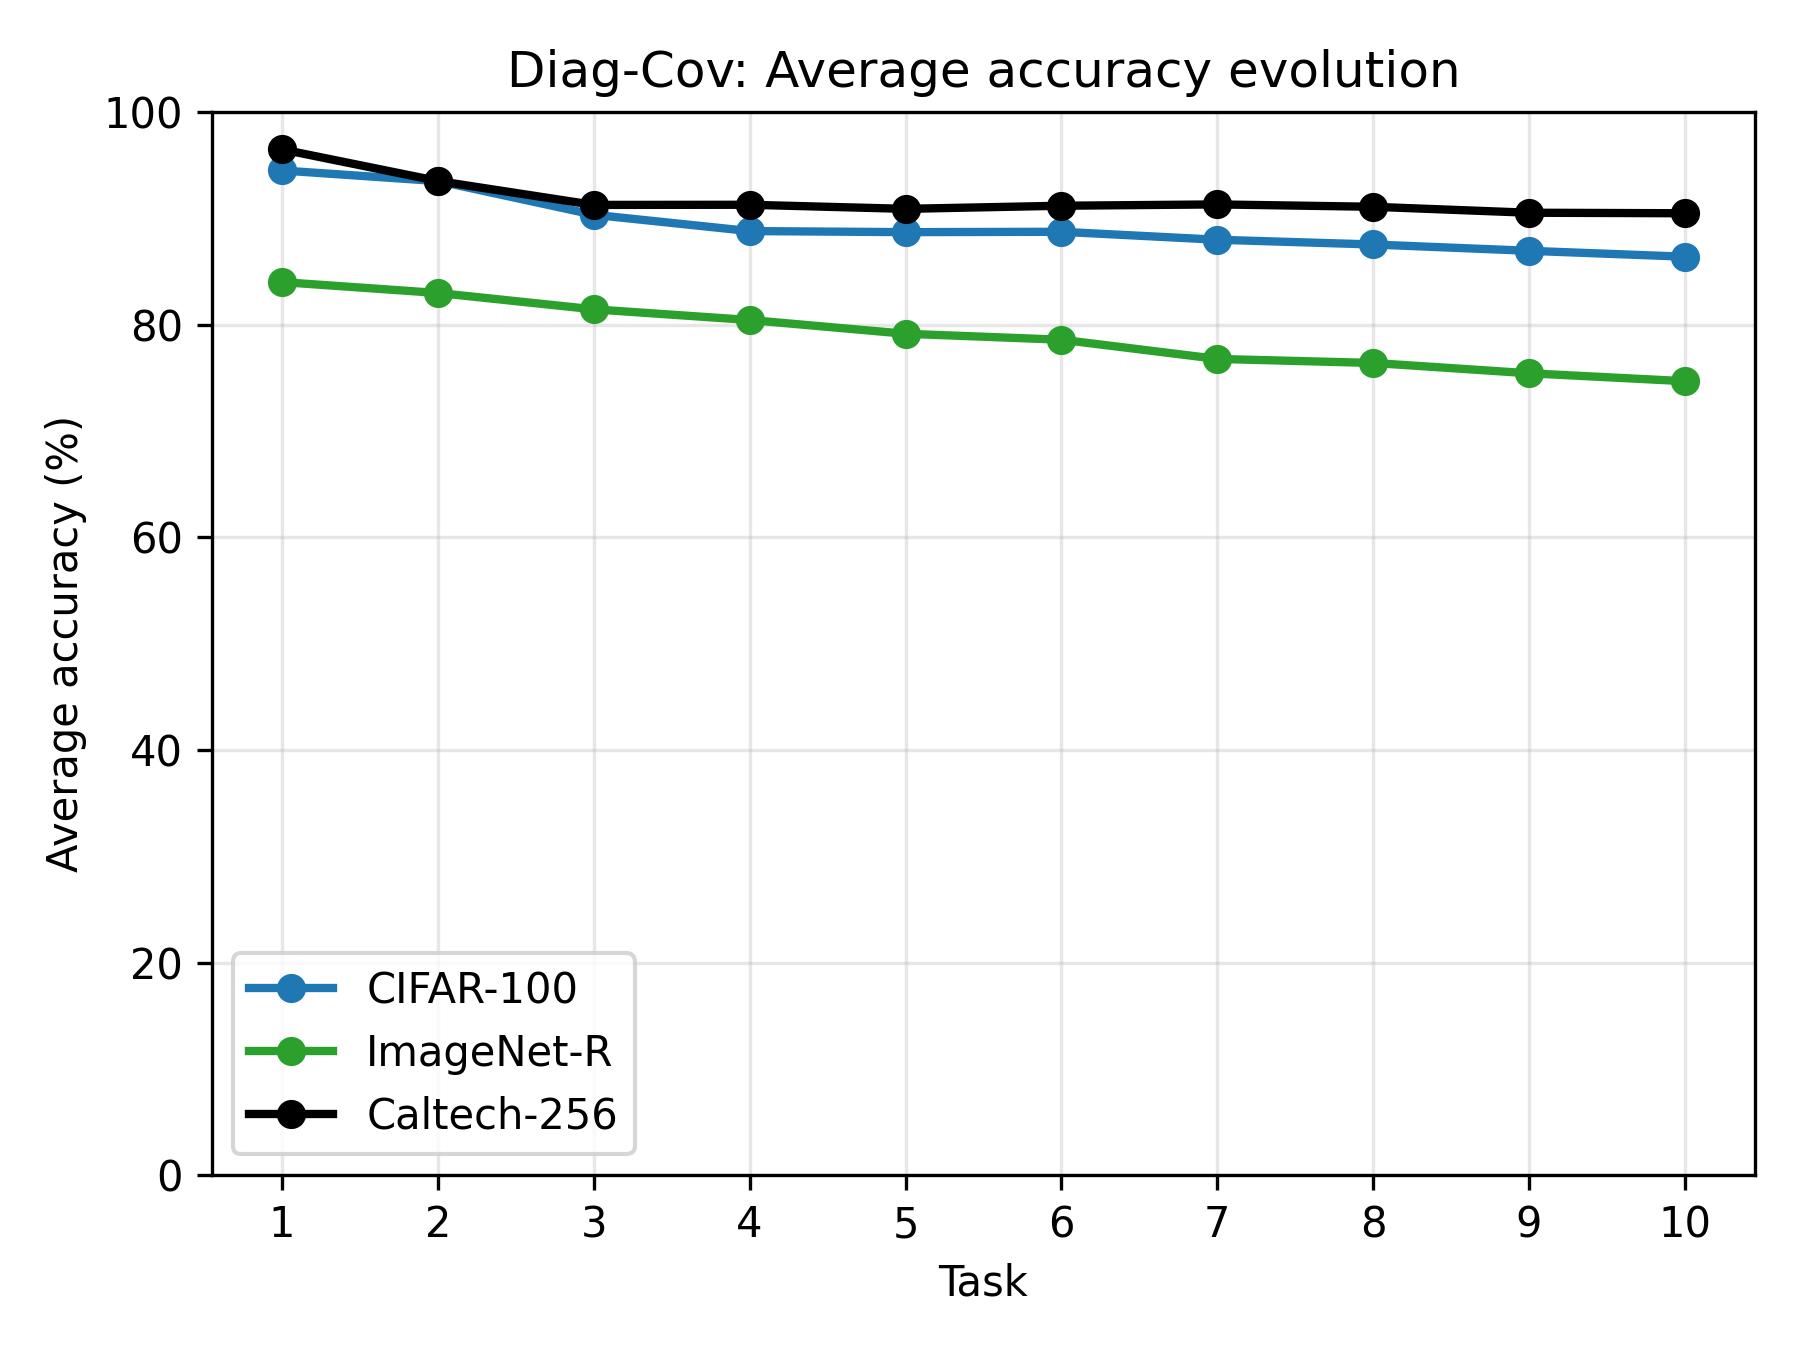
\includegraphics[width=0.32\linewidth]{imagenes/results/avg_accuracy_evolution_diagcov.png}}
	\hfill
	\subcaptionbox{Full-Cov}{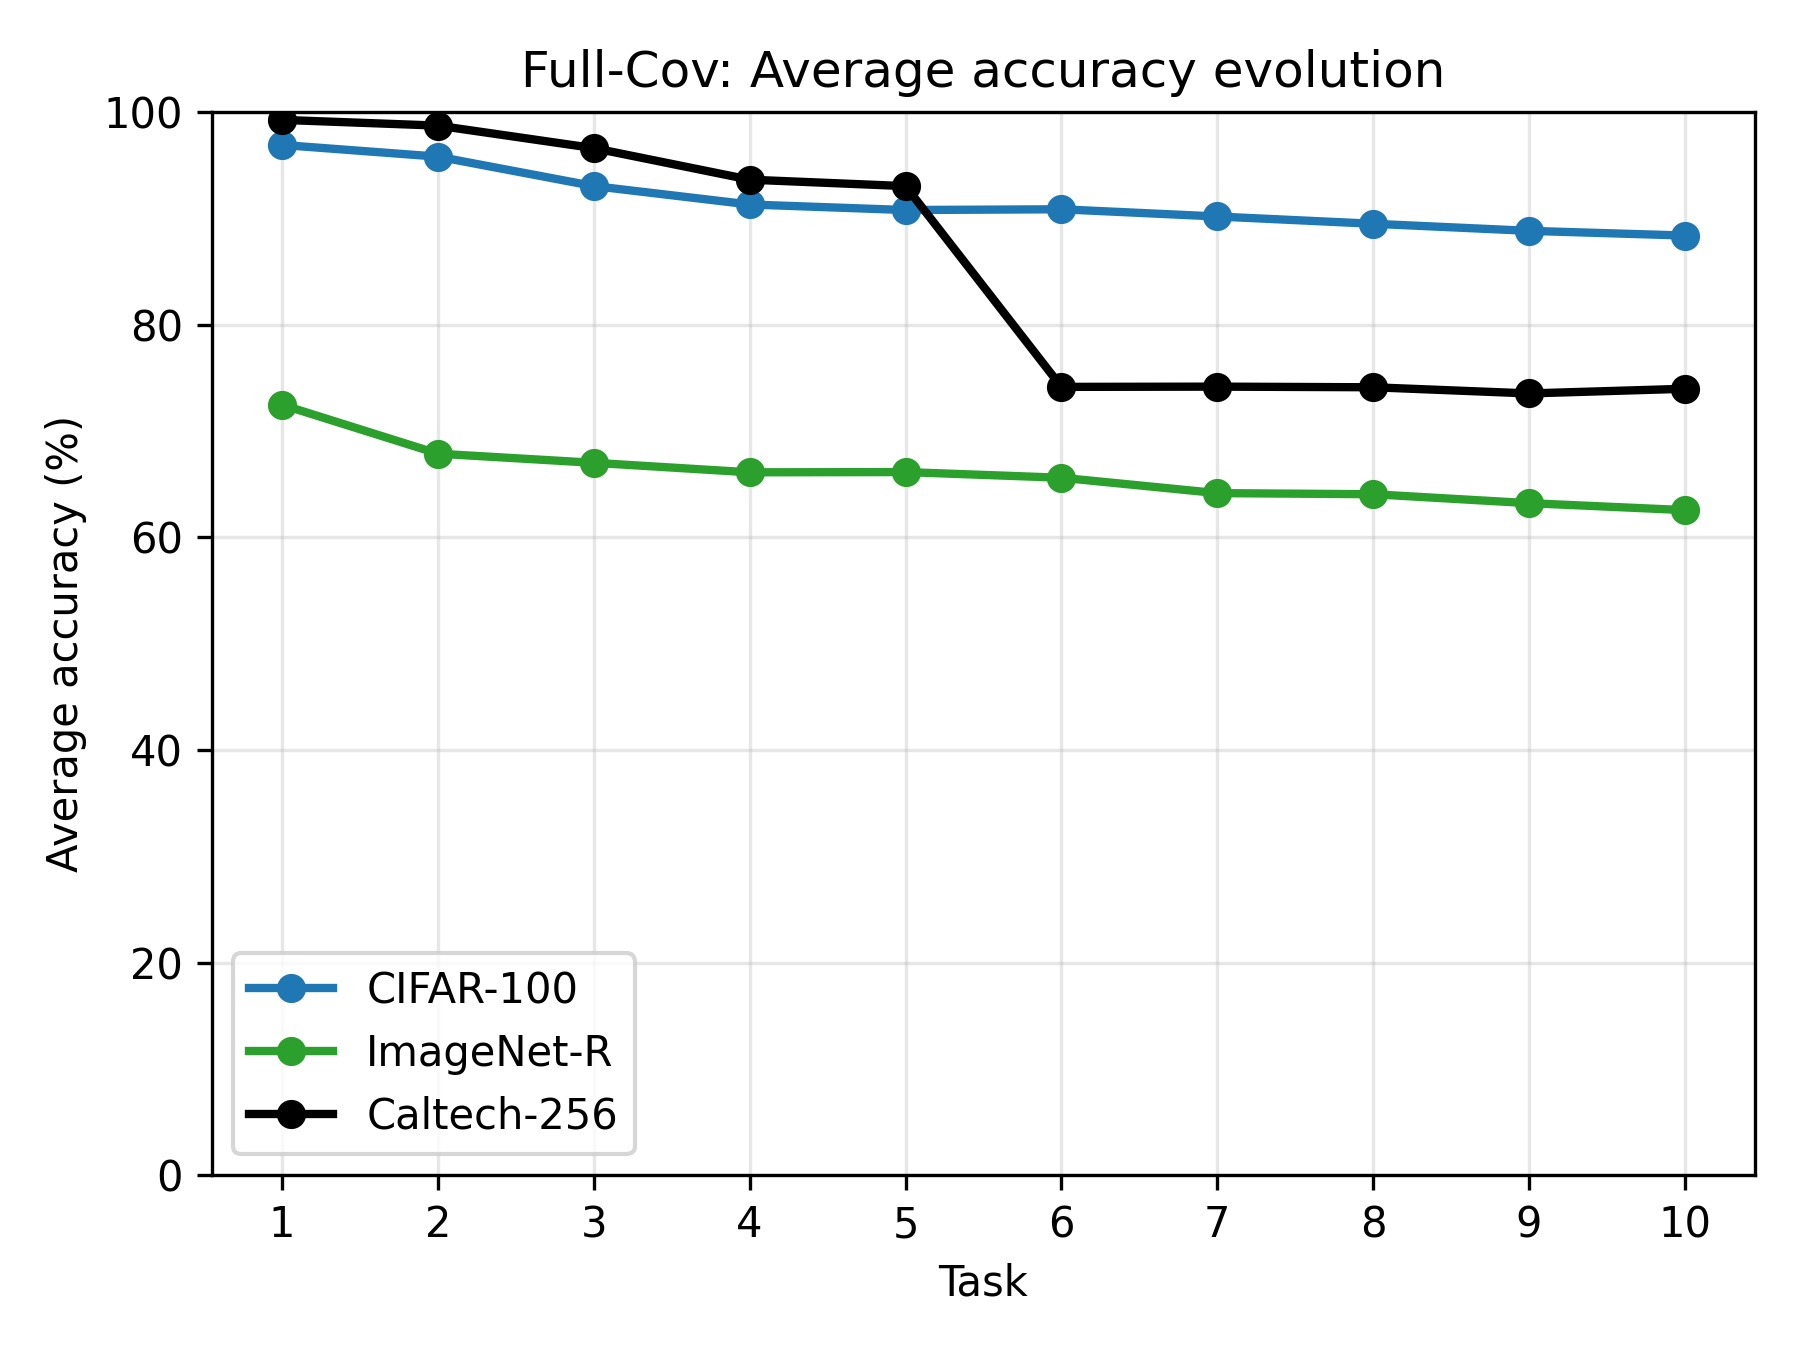
\includegraphics[width=0.32\linewidth]{imagenes/results/avg_accuracy_evolution_fullcov.png}}
	\hfill
	\subcaptionbox{MOG4-Shared}{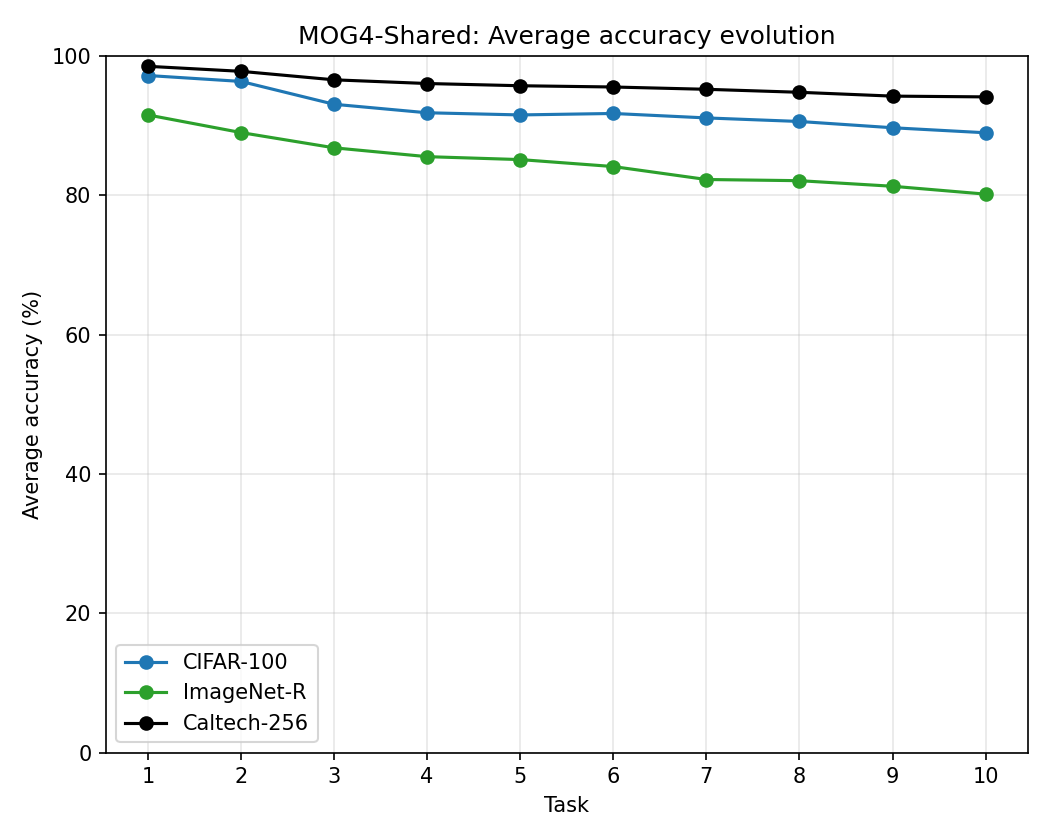
\includegraphics[width=0.32\linewidth]{imagenes/results/avg_accuracy_evolution_mog4shared.png}}
	\caption{Evolution of average accuracy across ten sequential tasks for CIFAR-100 (blue), ImageNet-R (green), and Caltech-256 (black), under (\textbf{a}) Diag-Cov, (\textbf{b}) Full-Cov, and (\textbf{c}) MOG4-Shared estimation.}
	\label{fig:avg_acc_evolution}
\end{figure}

This decline should not be read as forgetting in the usual sense. Every class-conditional Gaussian is estimated independently and frozen the moment its class is added, so no parameters from previously learned classes are ever overwritten: each class keeps, unchanged, the exact representation it was given when it was first learned. What grows with $t$ is not error on old classes caused by new ones, but the difficulty of the classification problem itself, since every extra task adds more competing prototypes for the Bayesian decision rule to tell apart. Figure~\ref{fig:bhattacharyya} quantifies this same mechanism through the decay of the minimum pairwise Bhattacharyya distance: as more classes are added, some pairs of prototypes inevitably move closer together in feature space, which raises the chance of confusion even though none of the individual class models has changed. The accuracy drop shown here is therefore a harder decision surface, not lost knowledge, and it matches the low forgetting values already reported in Table~\ref{tab:combined_benchmarks}. The next section develops this separability analysis in full.

\section{Inter-Class Separability}
\label{sec:interclass_results}

Before asking why some classes are harder than others, it helps to look at how accuracy is actually spread across classes once every one of them has been added to the stream. This section starts from that per-class picture, and then uses the geometry of the embedding space, through the Bhattacharyya and Euclidean distances between class prototypes, to explain why some classes end up harder to tell apart than others.

\subsection{Per-Class Accuracy Once All Classes Are Added}
\label{sec:an:recall_distributions}

Once every task has been added to the stream, the Diag-Cov classifier reaches overall accuracies of $86.6\%$, $90.2\%$, and $72.5\%$ on CIFAR-100, Caltech-256, and ImageNet-R respectively, while Full-Cov reaches $88.9\%$, $94.7\%$, and $74.7\%$ on those same benchmarks. Figures~\ref{fig:class_acc_hist_cifar}--\ref{fig:class_acc_hist_caltech} break these overall numbers down by class, showing how accuracy is actually spread across categories rather than being uniform.

\begin{figure}[htbp]
	\centering
	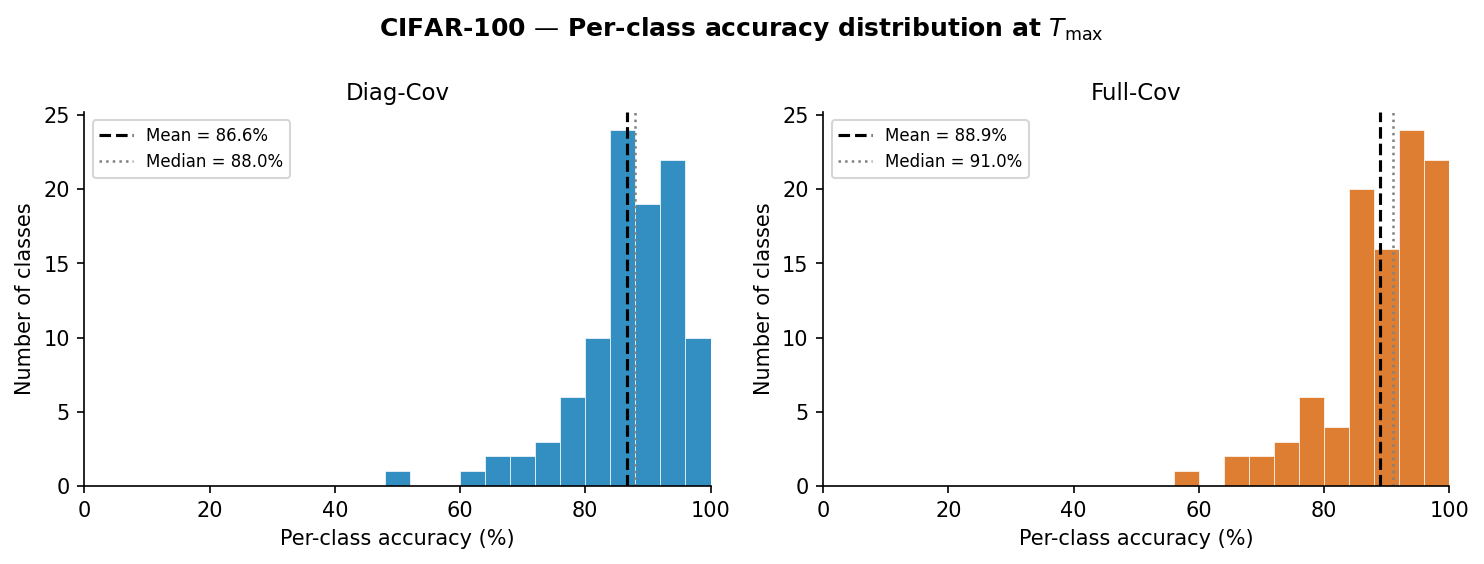
\includegraphics[width=0.99\linewidth]{imagenes/results/class_acc_hist_CIFAR100.png}
	\caption{Per-class accuracy once all classes have been added, for CIFAR-100 ($N=100$ classes). Left: Diag-Cov. Right: Full-Cov.}
	\label{fig:class_acc_hist_cifar}
\end{figure}

\begin{figure}[htbp]
	\centering
	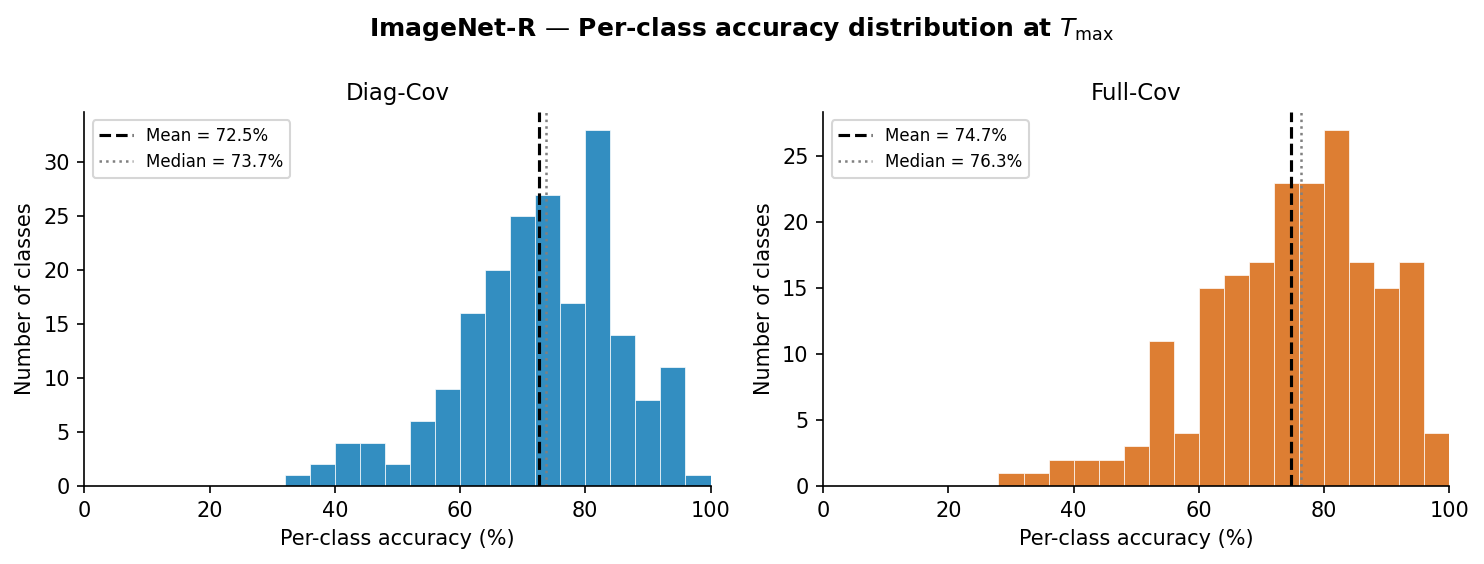
\includegraphics[width=0.99\linewidth]{imagenes/results/class_acc_hist_ImageNetR.png}
	\caption{Per-class accuracy once all classes have been added, for ImageNet-R ($N=200$ classes).}
	\label{fig:class_acc_hist_imagenetr}
\end{figure}

\begin{figure}[htbp]
	\centering
	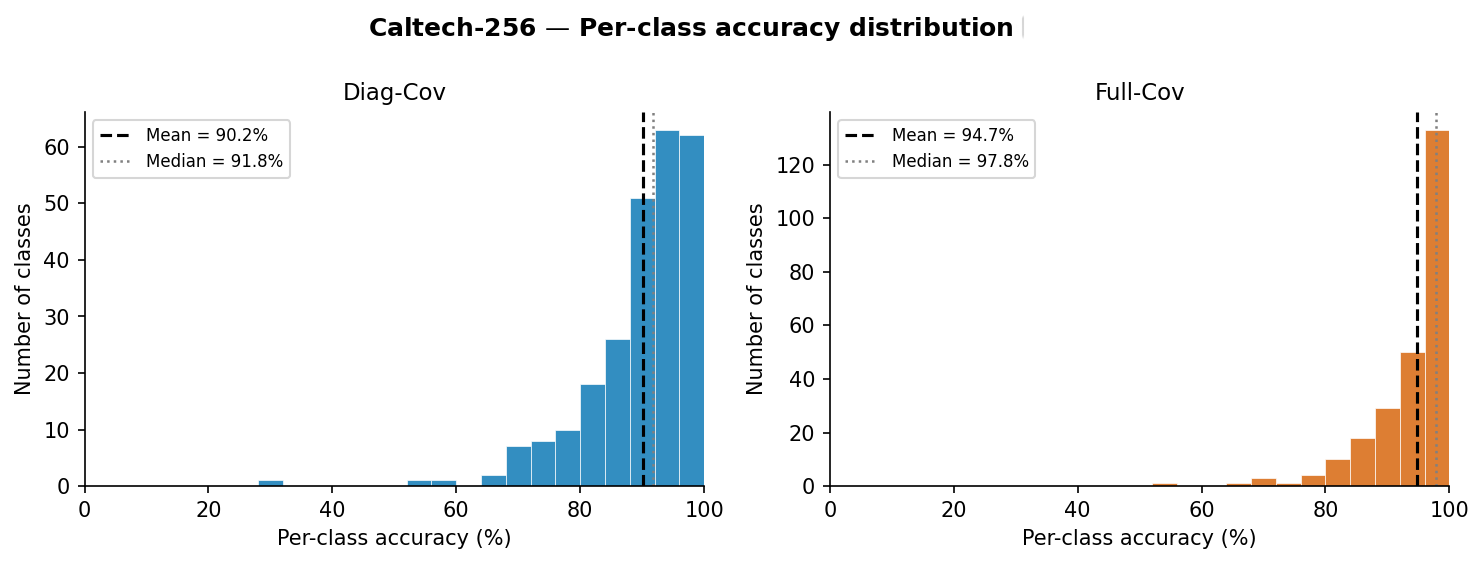
\includegraphics[width=0.99\linewidth]{imagenes/results/class_acc_hist_Caltech256.png}
	\caption{Per-class accuracy once all classes have been added, for Caltech-256 ($N=250$ classes).}
	\label{fig:class_acc_hist_caltech}
\end{figure}

The shapes of these histograms show two different pictures depending on the benchmark: on some, per-class accuracy is spread out across nearly the whole range, from very low to very high; on others, it stays tightly concentrated in one region. Either way, some classes always come out clearly better recognised than others.

On Split CIFAR-100, the recall profiles for both Diag-Cov and Full-Cov are tightly concentrated and broadly unimodal, skewed toward the highest accuracy bins. This concentration reflects the stable, well-behaved nature of low-resolution natural features, where most categories have compact feature distributions that single-component Gaussians approximate with little residual variance. Split Caltech-256 shows an even cleaner concentration peak; under Full-Cov estimation, the median shifts toward $97.8\%$, putting most of the dataset into a near-perfect recognition cluster. This shows that although high-resolution object photography introduces large variance across coordinates, its semantic categories occupy well isolated, linearly separable regions of the DINOv2 manifold, letting a full precision matrix separate the few remaining competitive boundaries.

Split ImageNet-R, by contrast, shows a dispersed, flat distribution with a long tail of low-accuracy classes extending down past the $40\%$ mark. Unlike the tight concentration seen in CIFAR-100 and Caltech-256, the visual features of ImageNet-R are not well concentrated. Because the imagery is intentionally out-of-distribution---spanning stylized art, cartoons, and hand-drawn sketches---the frozen foundation encoder maps these samples into broad, diffuse, and anisotropic representations. This lack of spatial concentration produces large intra-class variance and complex directional skewness, which limits the modeling capacity of single independent Gaussians.

As explained in Section~\ref{sec:incremental_update}, this gap between classes cannot come from forgetting in the usual sense: each class-conditional Gaussian is estimated once and frozen the moment its class is added, so nothing about how well an old class is modelled can change afterwards. If some classes still end up much harder than others once every task has been seen, the cause has to be something else, namely how close different classes actually sit to each other in the embedding space. The rest of this section looks at that directly.

\subsection{Class Overlap: Bhattacharyya and Euclidean Distances}
\label{sec:an:interclass}

To see how close different classes sit to each other in the embedding space, we use two complementary measures: the \emph{Bhattacharyya distance} $D_B$, which accounts for differences in both class means and covariances, and the plain \emph{Euclidean distance} $d_E = \|\boldsymbol{\mu}_i - \boldsymbol{\mu}_j\|_2$ between class mean vectors, which isolates mean separation alone.

\begin{figure}[htbp]
	\centering
	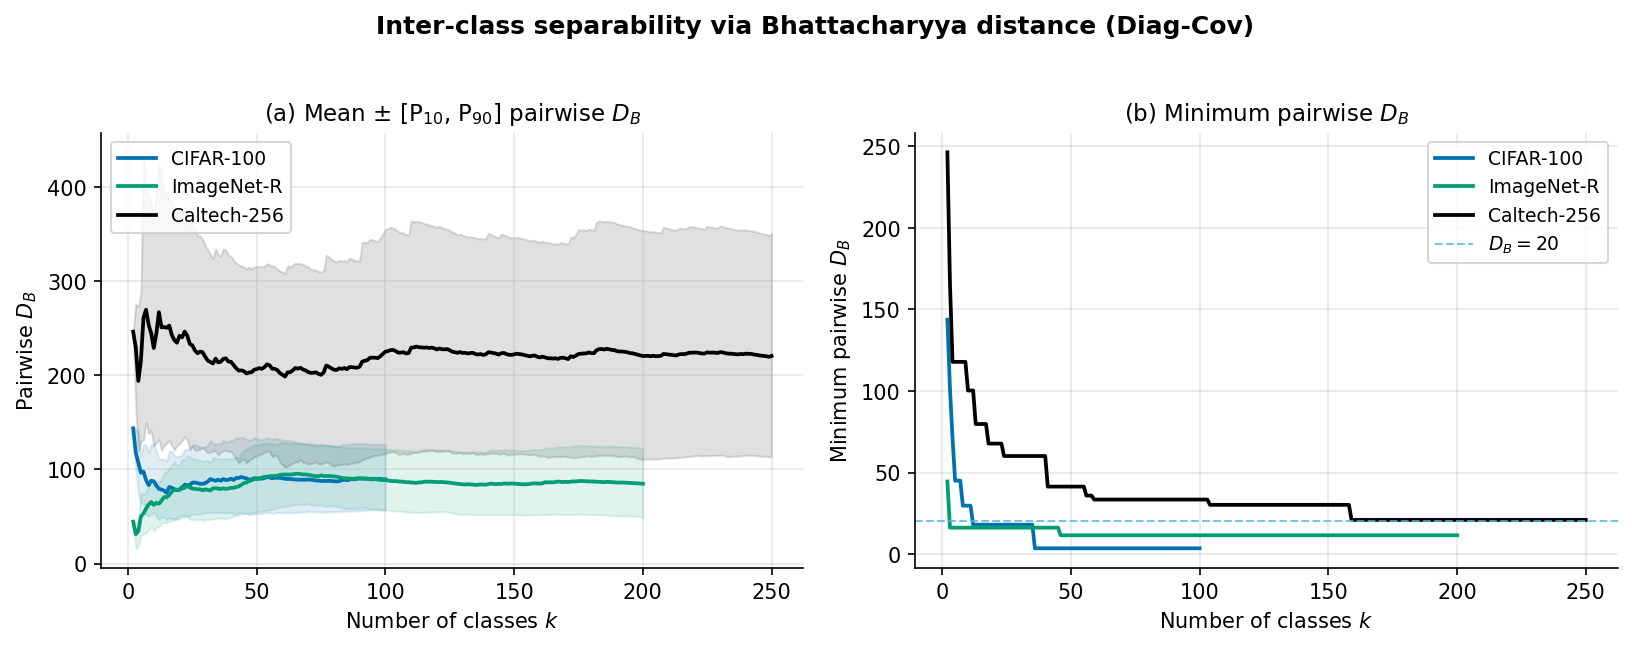
\includegraphics[width=0.99\linewidth]{imagenes/results/bhattacharyya_ab.png}
	\caption{%
		Inter-class separability under the Diag-Cov Gaussian model as the class
		set grows from $k=2$ to the full benchmark size.
		\textbf{(a)}~Mean pairwise $D_B$ with shaded $[\mathrm{P}_{10},\mathrm{P}_{90}]$ band.
		\textbf{(b)}~Minimum pairwise $D_B$; the dashed horizontal line marks $D_B\!=\!20$.%
	}
	\label{fig:bhattacharyya}
\end{figure}

\begin{figure}[htbp]
	\centering
	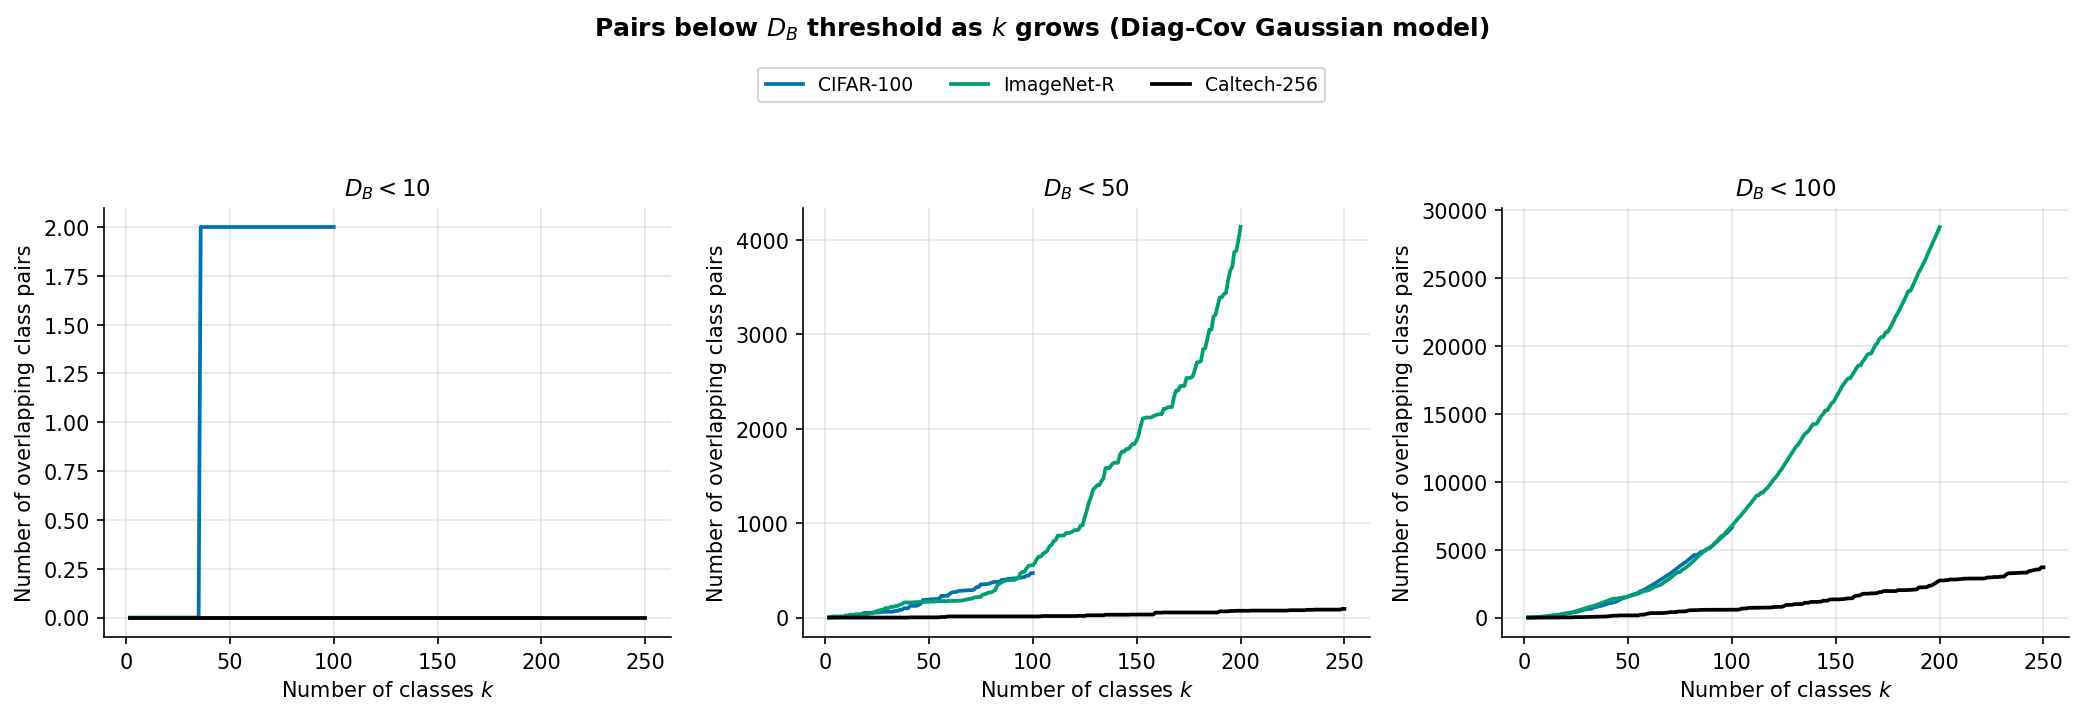
\includegraphics[width=0.99\linewidth]{imagenes/results/bhattacharyya_thresholds.png}
	\caption{%
		Count of class pairs below three overlap thresholds ($D_B < 10$, $D_B < 50$,
		$D_B < 100$) as the class set grows. Over $99.8\,\%$ of all pairs exceed
		$D_B\!=\!50$ on every benchmark.%
	}
	\label{fig:bhattacharyya_thresholds}
\end{figure}

\begin{figure}[htbp]
	\centering
	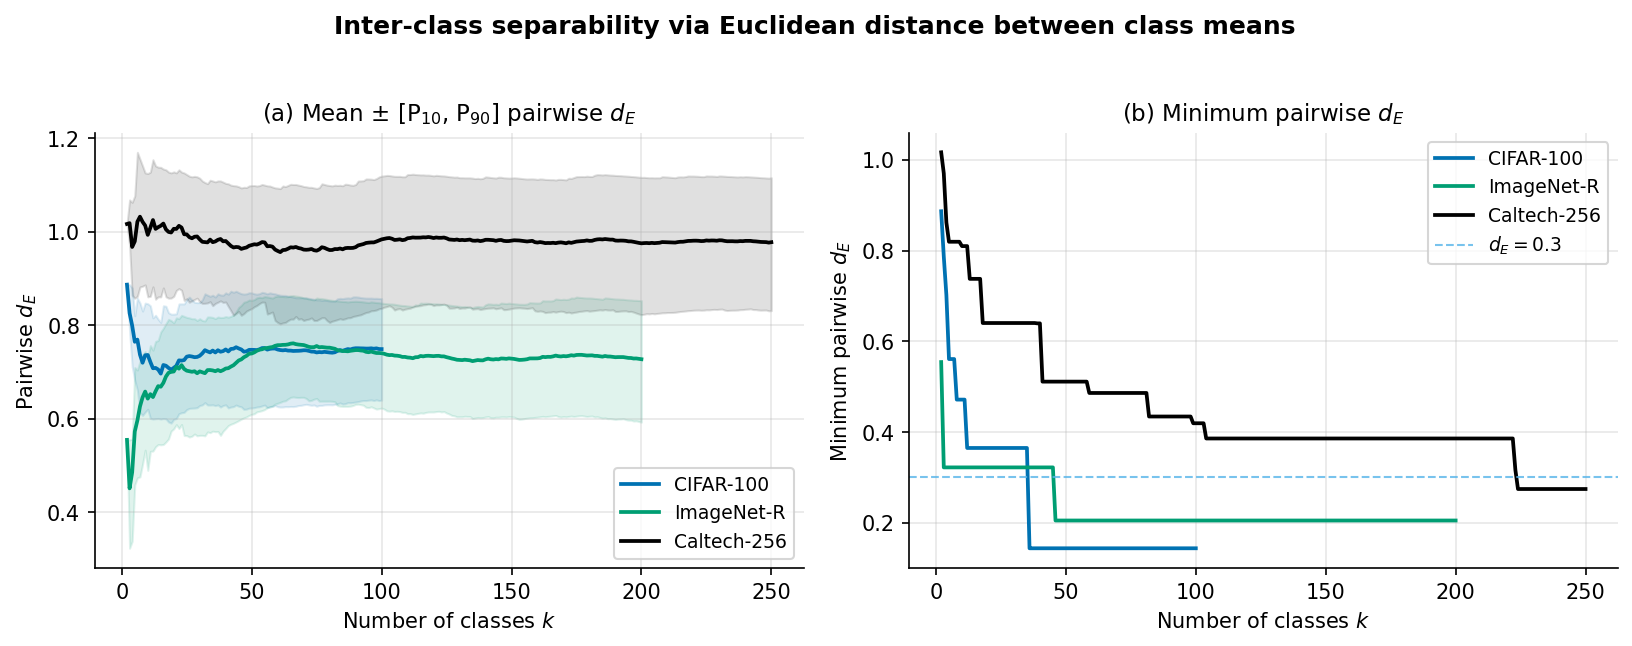
\includegraphics[width=0.99\linewidth]{imagenes/results/euclidean_ab.png}
	\caption{%
		Inter-class separability in terms of the plain Euclidean distance
		$d_E$ between class means, as the class set grows from $k=2$ to the
		full benchmark size.
		\textbf{(a)}~Mean pairwise $d_E$ with shaded $[\mathrm{P}_{10},\mathrm{P}_{90}]$ band.
		\textbf{(b)}~Minimum pairwise $d_E$.%
	}
	\label{fig:euclidean}
\end{figure}

\begin{figure}[htbp]
	\centering
	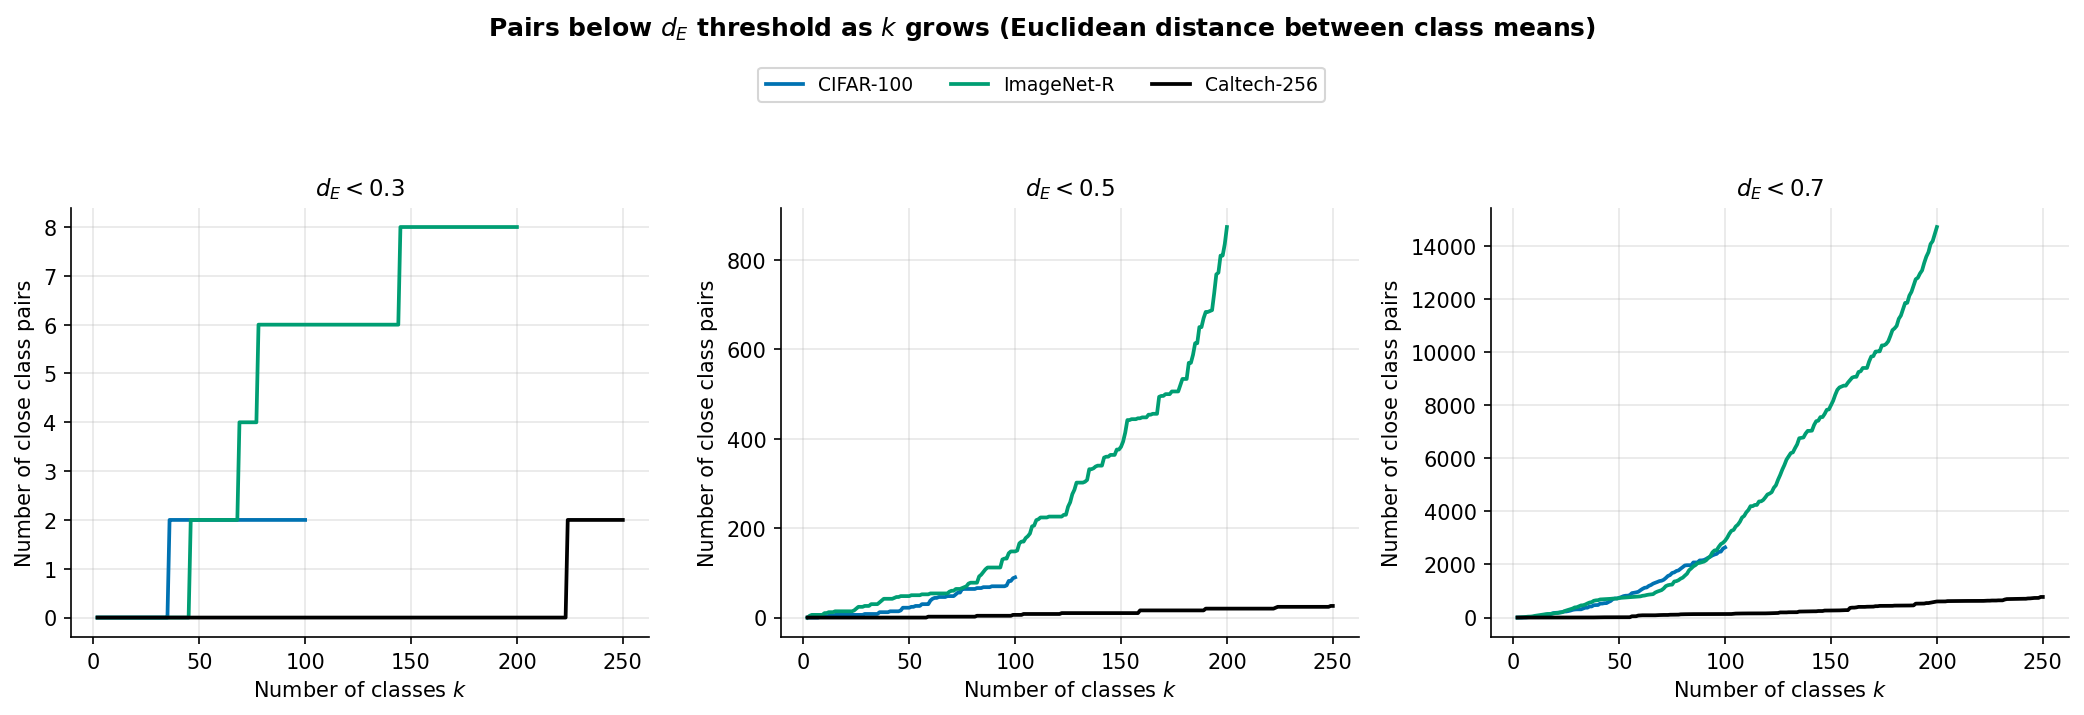
\includegraphics[width=0.99\linewidth]{imagenes/results/euclidean_thresholds.png}
	\caption{%
		Count of class pairs below three Euclidean-distance overlap thresholds
		as the class set grows, complementing the Bhattacharyya-based count of
		Figure~\ref{fig:bhattacharyya_thresholds}.%
	}
	\label{fig:euclidean_thresholds}
\end{figure}

The scaling trajectories of the pairwise Bhattacharyya distances (Figures~\ref{fig:bhattacharyya} and~\ref{fig:bhattacharyya_thresholds}) and mean Euclidean distances (Figures~\ref{fig:euclidean} and~\ref{fig:euclidean_thresholds}) show a consistent pattern across the foundation embedding manifolds. Rather than an overall compression of the representation space as tasks accumulate, the global layout of the features stays fairly stable, while performance is limited mainly by a small, heavy-tailed set of overlapping class pairs.

One sign of this stability is that both macro-averaged distance metrics plateau quickly across all benchmarks once around 30 categories are introduced. At full class-set size, the mean pairwise $D_B$ settles at $220.61$ for Caltech-256, $89.43$ for CIFAR-100, and $84.81$ for ImageNet-R. This same ordering is matched by the macro-averaged mean Euclidean distance, where Caltech-256 keeps a wide geometric separation of $\overline{d_E} = 0.978$, while CIFAR-100 and ImageNet-R stay more densely packed at $\overline{d_E} = 0.749$ and $\overline{d_E} = 0.727$, respectively. Caltech-256's clear separability advantage on both metrics reflects its greater visual and semantic diversity, which keeps per-class distributions distinct.

However, as the label space grows denser, the minimum pairwise distance metrics decay steadily, and this is the real driver behind the accuracy gaps between classes seen in the previous subsection. Once every class has been added, the minimum pairwise $D_B$ drops to $3.57$ on CIFAR-100, $11.54$ on ImageNet-R, and $20.96$ on Caltech-256. This localized crowding is confirmed by the Euclidean mean separation, which hits minimum values of $0.144$, $0.205$, and $0.275$ for the respective datasets.

Tracking the density thresholds shows that this crowding is an isolated effect rather than a general collapse of the space. Over $99.8\,\%$ of all possible class combinations stay well above a threshold of $D_B = 50$ on every evaluated benchmark. Similarly, class pairs with $d_E < 0.5$ make up only a small fraction of the total, accounting for $0.91\,\%$ of pairs in CIFAR-100, $2.20\,\%$ in ImageNet-R, and just $0.04\,\%$ in Caltech-256.

So the classifier is not working in a uniformly collapsed or muddy feature space. Instead, the accuracy ceilings ($88.87\%$ for CIFAR-100, $77.99\%$ for ImageNet-R, and $94.36\%$ for Caltech-256 under the strongest Gaussian configurations) are set by a small number of highly confusable prototype pairs, which is exactly what produces the long low-accuracy tail seen on ImageNet-R in the previous subsection.

The two metrics act as complementary diagnostics for these failure points. While $d_E$ isolates pure first-order geometric separation between prototype centroids, $D_B$ also penalizes covariance shape and volume differences. This explains why a pair such as \textit{boy}/\textit{girl} in CIFAR-100 stands out as the single biggest source of confusion in the system: it combines a very small geometric centroid distance ($d_E = 0.145$) with nearly identical, overlapping second-order covariance structures, pushing the probabilistic separation down to its minimum. To see exactly which classes this affects and why, we now look at individual class confusion patterns, examining the visual and geometric identities of the worst-performing classes in the system.

\subsection{Worst-Performing Classes and Failure Diagnostics}
\label{sec:worst_classes}

Breaking macro-level performance metrics down into class-specific failure points gives a clearer view of the resolution limits of the visual foundation embedding space and the boundaries of each covariance parameterisation. To isolate these failure cases, we rank and track the five object categories with the lowest per-class recall scores across all benchmarks.

We analyze these failure patterns across two parameterisations: Table~\ref{tab:worst_diag} characterizes the five lowest-performing classes under the independent feature assumptions of the Diagonal Covariance model, while Table~\ref{tab:worst_full} evaluates the corresponding distribution shifts and re-orderings under the regularized Full Covariance parameterisation. For both, the table records the empirical recall, the dominant confusion sink, the localized pairwise Bhattacharyya distance ($D_B$), and the Euclidean distance ($d_E$) to that primary target. These are compared directly against the dataset-level macro-averaged distances ($\overline{D_B}$ and $\overline{d_E}$) established in Section~\ref{sec:an:interclass}. Localized metrics falling well below these macro-averages give a direct geometric indication of significant prototype overlap.

\begin{table}[htbp]
	\centering
	\small
	\caption{Analysis of the five lowest-recall classes on each benchmark under Diagonal Covariance (Diag-Cov). $\text{Conf.}\%$ represents the percentage of errors directed toward the main confusion target. $D_B$ and $d_E$ denote the pairwise Bhattacharyya and Euclidean distances to the main confusion target, respectively, while $\overline{D_B}$ and $\overline{d_E}$ represent the macro-averaged pairwise distances across the entire dataset split.}
	\label{tab:worst_diag}
	\begin{adjustbox}{width=0.95\columnwidth, center}
		\small
		\begin{tabular}{llccccccc}
			\toprule
			\textbf{Dataset} & \textbf{Class} & \textbf{Acc\%} & \textbf{Main Confusion} & \textbf{Conf.\%} & $D_B$ & $\overline{D_B}$ & $d_E$ & $\overline{d_E}$ \\
			\midrule
			\textbf{Split CIFAR-100}
			& \textit{boy}          & 50.0 & \textit{girl}       & 30.0 &   3.45 & 89.43 & 0.145 & 0.749 \\
			& \textit{maple\_tree} & 60.0 & \textit{oak\_tree}  & 19.0 & 19.41 & 89.43 & 0.327 & 0.749 \\
			& \textit{girl}         & 65.0 & \textit{boy}        & 23.0 &   3.45 & 89.43 & 0.145 & 0.749 \\
			& \textit{cloud}        & 65.0 & \textit{sea}        &  8.0 & 30.54 & 89.43 & 0.451 & 0.749 \\
			& \textit{shrew}        & 69.0 & \textit{mouse}      & 16.0 & 16.45 & 89.43 & 0.331 & 0.749 \\
			\midrule
			\textbf{Split ImageNet-R}
			& \textit{cabbage}        & 35.3 & \textit{vase}           & 17.6 & 50.50 & 84.81 & 0.587 & 0.727 \\
			& \textit{saint\_bernard} & 36.4 & \textit{basset\_hound}  &  9.1 & 66.44 & 84.81 & 0.643 & 0.727 \\
			& \textit{bow\_tie}       & 39.3 & \textit{scarf}          & 21.4 & 16.57 & 84.81 & 0.331 & 0.727 \\
			& \textit{beaver}         & 40.0 & \textit{backpack}       &  8.6 & 34.74 & 84.81 & 0.500 & 0.727 \\
			& \textit{bee}            & 41.6 & \textit{fly}            & 15.6 & 20.51 & 84.81 & 0.378 & 0.727 \\
			\midrule
			\textbf{Split Caltech-256}
			& \textit{top-hat}        & 31.2 & \textit{cowboy-hat}     & 31.2 & 29.75 & 220.61 & 0.319 & 0.978 \\
			& \textit{paperclip}      & 52.6 & \textit{drinking-straw} & 21.1 & 62.94 & 220.61 & 0.645 & 0.978 \\
			& \textit{canoe}          & 57.1 & \textit{people}         & 28.6 & 57.87 & 220.61 & 0.641 & 0.978 \\
			& \textit{drinking-straw} & 64.7 & \textit{people}         & 11.8 & 27.33 & 220.61 & 0.465 & 0.978 \\
			& \textit{traffic-light}  & 65.0 & \textit{people}         & 15.0 & 66.27 & 220.61 & 0.675 & 0.978 \\
			\bottomrule
		\end{tabular}
	\end{adjustbox}
\end{table}

Table~\ref{tab:worst_full} details the equivalent classification landscapes under the regularized Full Covariance model. While the low-recall sets overlap heavily on the localized natural structures of Split CIFAR-100, they diverge substantially on the high-resolution object coordinates of Split Caltech-256. Because $\overline{D_B}$ and $\overline{d_E}$ represent fundamental global properties of the static underlying feature distributions, they remain identical to the baseline values reported in Table~\ref{tab:worst_diag}. 

\begin{table}[htbp]
	\centering
	\small
	\caption{Analysis of the five lowest-recall classes on each benchmark under Full Covariance (Full-Cov). Columns match the structure of Table~\ref{tab:worst_diag}; the probabilistic distance $D_B$ is computed using the regularized diagonal components for numeric consistency across the imbalanced stream.}
	\label{tab:worst_full}
	\begin{adjustbox}{width=0.95\columnwidth, center}
		\small
		\begin{tabular}{llccccccc}
			\toprule
			\textbf{Dataset} & \textbf{Class} & \textbf{Acc\%} & \textbf{Main Confusion} & \textbf{Conf.\%} & $D_B$ & $\overline{D_B}$ & $d_E$ & $\overline{d_E}$ \\
			\midrule
			\textbf{Split CIFAR-100}
			& \textit{boy}          & 58.0 & \textit{girl}       & 16.0 &   3.45 & 89.43 & 0.145 & 0.749 \\
			& \textit{girl}         & 67.0 & \textit{boy}        & 15.0 &   3.45 & 89.43 & 0.145 & 0.749 \\
			& \textit{otter}        & 67.0 & \textit{seal}       &  8.0 & 16.42 & 89.43 & 0.342 & 0.749 \\
			& \textit{maple\_tree} & 68.0 & \textit{oak\_tree}  & 19.0 & 19.41 & 89.43 & 0.327 & 0.749 \\
			& \textit{forest}       & 68.0 & \textit{pine\_tree} &  7.0 & 25.46 & 89.43 & 0.422 & 0.749 \\
			\midrule
			\textbf{Split ImageNet-R}
			& \textit{bow\_tie}    & 28.6 & \textit{cowboy\_hat} & 14.3 & 14.51 & 84.81 & 0.323 & 0.727 \\
			& \textit{bee}          & 33.8 & \textit{fly}        & 11.7 & 20.51 & 84.81 & 0.378 & 0.727 \\
			& \textit{beaver}       & 37.1 & \textit{backpack}   &  8.6 & 34.74 & 84.81 & 0.500 & 0.727 \\
			& \textit{cowboy\_hat} & 39.0 & \textit{hammer}     &  6.8 & 21.01 & 84.81 & 0.404 & 0.727 \\
			& \textit{candle}       & 40.7 & \textit{stole}      &  9.3 & 19.73 & 84.81 & 0.379 & 0.727 \\
			\midrule
			\textbf{Split Caltech-256}
			& \textit{drinking-straw}  & 52.9 & \textit{soda-can}     & 11.8 &  51.11 & 220.61 & 0.614 & 0.978 \\
			& \textit{people}          & 66.7 & \textit{picnic-table} &  4.8 &  55.38 & 220.61 & 0.619 & 0.978 \\
			& \textit{top-hat}          & 68.8 & \textit{wine-bottle}  &  6.2 & 100.90 & 220.61 & 0.802 & 0.978 \\
			& \textit{american-flag}   & 70.0 & \textit{speed-boat}   &  5.0 & 108.32 & 220.61 & 0.823 & 0.978 \\
			& \textit{bowling-ball}    & 71.4 & \textit{bowling-pin}  & 14.3 &  68.73 & 220.61 & 0.644 & 0.978 \\
			\bottomrule
		\end{tabular}
	\end{adjustbox}
\end{table}

To ground these proximity numbers in something visual, we look at typical images taken directly from the benchmark data streams. Figures~\ref{fig:worst_repr_cifar}, \ref{fig:worst_repr_imagenetr}, and~\ref{fig:worst_repr_caltech} present the target classes side by side with their main cross-category confusion partners, the samples most frequently confused by the classifier. Looking at these cross-class pairs shows the structural and semantic similarities that drive the lower tails of our recall curves.

% ==========================================
% FIGURE 1: CIFAR-100 (4x2 Grid) - FIXED
% ==========================================
\begin{figure}[htbp]
	\centering
	
	% --- Row 1 ---
	\begin{minipage}[t]{0.23\linewidth}
		\centering
		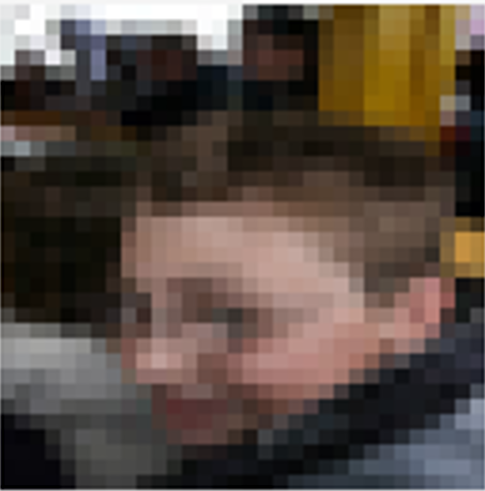
\includegraphics[width=0.99\linewidth]{imagenes/results/cifar_100/boy.png}\\
		{\small (a) Boy}
	\end{minipage}\hfill
	\begin{minipage}[t]{0.23\linewidth}
		\centering
		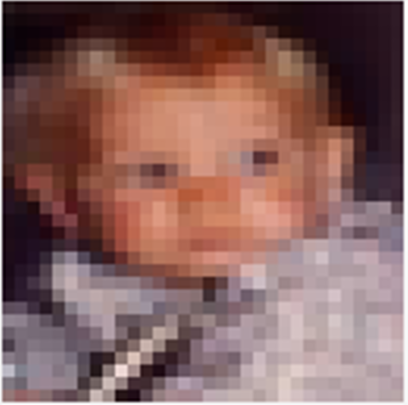
\includegraphics[width=0.99\linewidth]{imagenes/results/cifar_100/girl.png}\\
		{\small (b) Girl}
	\end{minipage}\hfill
	\begin{minipage}[t]{0.23\linewidth}
		\centering
		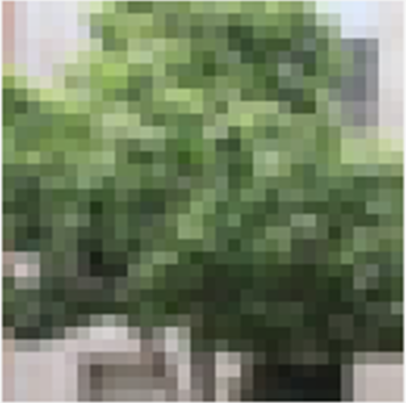
\includegraphics[width=0.99\linewidth]{imagenes/results/cifar_100/oak_tree.png}\\
		{\small (c) Oak Tree}
	\end{minipage}\hfill
	\begin{minipage}[t]{0.23\linewidth}
		\centering
		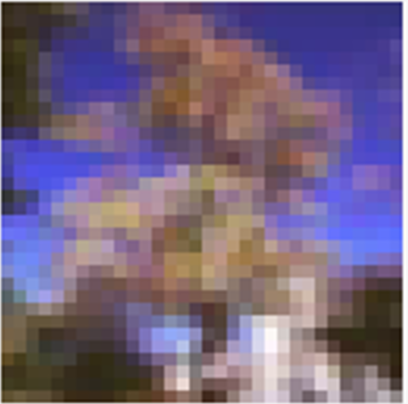
\includegraphics[width=0.99\linewidth]{imagenes/results/cifar_100/maple_tree.png}\\
		{\small (d) Maple Tree}
	\end{minipage}
	
	\vspace{0.4cm}
	
	% --- Row 2 ---
	\begin{minipage}[t]{0.23\linewidth}
		\centering
		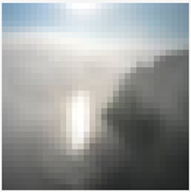
\includegraphics[width=0.99\linewidth]{imagenes/results/cifar_100/cloud.png}\\
		{\small (e) Cloud}
	\end{minipage}\hfill
	\begin{minipage}[t]{0.23\linewidth}
		\centering
		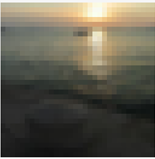
\includegraphics[width=0.99\linewidth]{imagenes/results/cifar_100/sea.png}\\
		{\small (f) Sea}
	\end{minipage}\hfill
	\begin{minipage}[t]{0.23\linewidth}
		\centering
		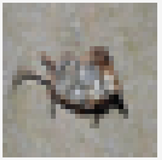
\includegraphics[width=0.99\linewidth]{imagenes/results/cifar_100/shrew.png}\\
		{\small (g) Shrew}
	\end{minipage}\hfill
	\begin{minipage}[t]{0.23\linewidth}
		\centering
		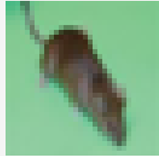
\includegraphics[width=0.99\linewidth]{imagenes/results/cifar_100/mouse.png}\\
		{\small (h) Mouse}
	\end{minipage}
	
	\caption{Representative visual specimens of the primary low-recall classes and corresponding confusion sinks on the Split CIFAR-100 benchmark, mapped to the tracking trends outlined in Table~\ref{tab:worst_diag} and Table~\ref{tab:worst_full}.}
	\label{fig:worst_repr_cifar}
\end{figure}

% ==========================================
% FIGURE 2: ImageNet-R (5x2 Grid)
% ==========================================
\begin{figure}[htbp]
	\centering
	
	% --- Row 1: First 5 images ---
	\begin{minipage}[t]{0.18\linewidth}
		\centering
		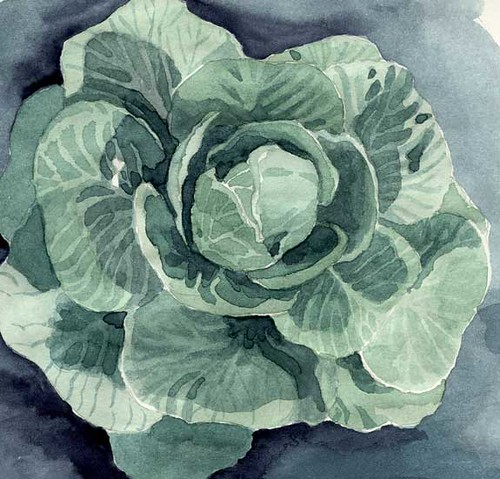
\includegraphics[width=0.9\linewidth]{imagenes/results/imagenetr/cabbage.jpg}\\
		{\small (a) Cabbage}
	\end{minipage}\hfill
	\begin{minipage}[t]{0.18\linewidth}
		\centering
		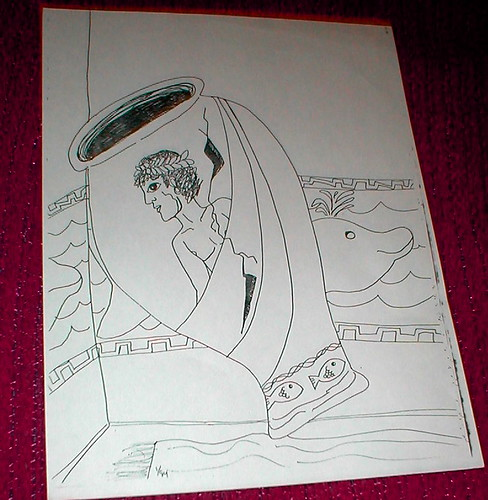
\includegraphics[width=0.9\linewidth]{imagenes/results/imagenetr/vase.jpg}\\
		{\small (b) Vase}
	\end{minipage}\hfill
	\begin{minipage}[t]{0.18\linewidth}
		\centering
		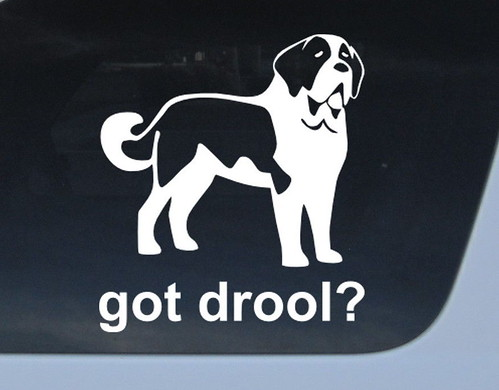
\includegraphics[width=0.9\linewidth]{imagenes/results/imagenetr/saint_bernard.jpg}\\
		{\small (c) Saint Bernard}
	\end{minipage}\hfill
	\begin{minipage}[t]{0.18\linewidth}
		\centering
		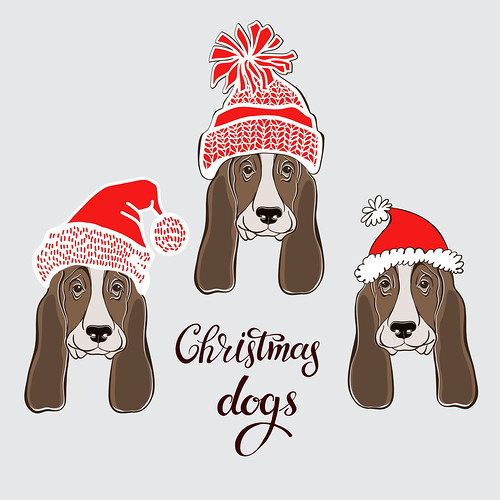
\includegraphics[width=0.9\linewidth]{imagenes/results/imagenetr/basset_hound.jpg}\\
		{\small (d) Basset Hound}
	\end{minipage}\hfill
	\begin{minipage}[t]{0.18\linewidth}
		\centering
		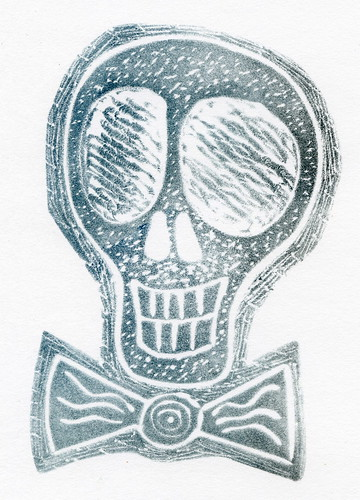
\includegraphics[width=0.9\linewidth]{imagenes/results/imagenetr/bow_tie.jpg}\\
		{\small (e) Bow Tie}
	\end{minipage}
	
	\vspace{0.4cm}
	
	% --- Row 2: Remaining 5 images ---
	\begin{minipage}[t]{0.18\linewidth}
		\centering
		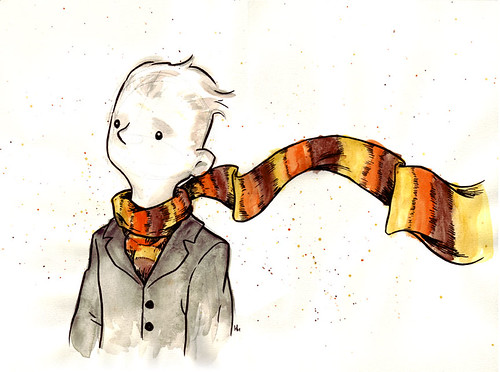
\includegraphics[width=0.9\linewidth]{imagenes/results/imagenetr/scarf.jpg}\\
		{\small (f) Scarf}
	\end{minipage}\hfill
	\begin{minipage}[t]{0.18\linewidth}
		\centering
		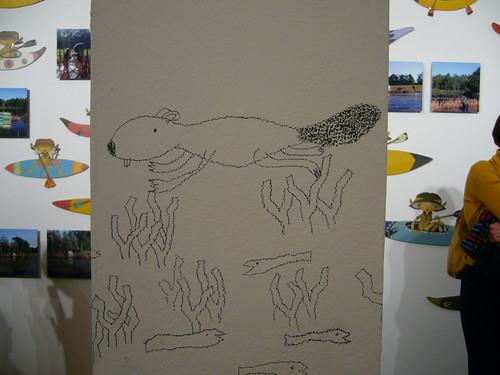
\includegraphics[width=0.9\linewidth]{imagenes/results/imagenetr/beaver.jpg}\\
		{\small (g) Beaver}
	\end{minipage}\hfill
	\begin{minipage}[t]{0.18\linewidth}
		\centering
		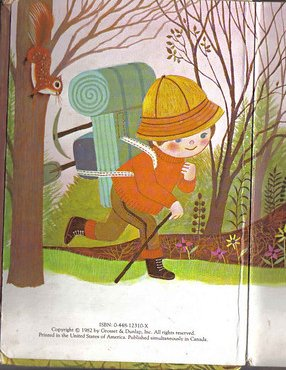
\includegraphics[width=0.9\linewidth]{imagenes/results/imagenetr/backpack.jpg}\\
		{\small (h) Backpack}
	\end{minipage}\hfill
	\begin{minipage}[t]{0.18\linewidth}
		\centering
		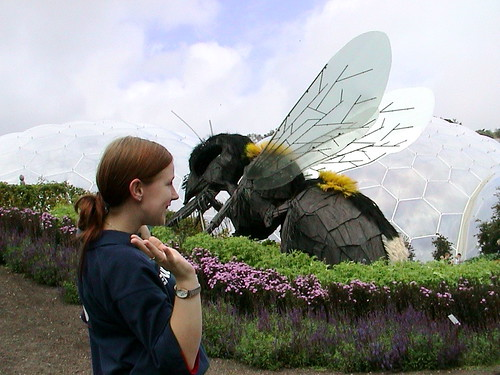
\includegraphics[width=0.9\linewidth]{imagenes/results/imagenetr/bee.jpg}\\
		{\small (i) Bee}
	\end{minipage}\hfill
	\begin{minipage}[t]{0.18\linewidth}
		\centering
		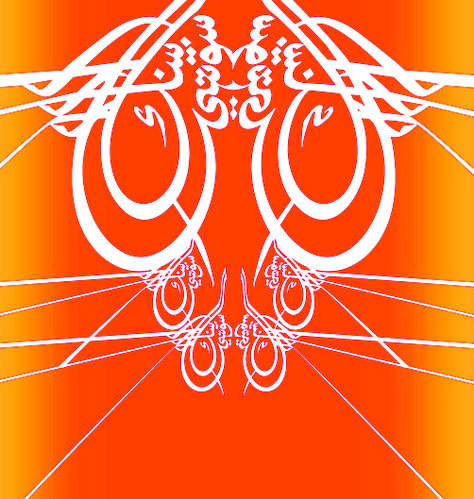
\includegraphics[width=0.9\linewidth]{imagenes/results/imagenetr/fly.jpg}\\
		{\small (j) Fly}
	\end{minipage}
	
	\caption{Representative specimens from Split ImageNet-R mapped to the tracking trends outlined in Table~\ref{tab:worst_diag} and Table~\ref{tab:worst_full}, showing the non-photographic style of the dataset.}
	\label{fig:worst_repr_imagenetr}
\end{figure}

% ==========================================
% FIGURE 3: Caltech-256 (4 + 3 Centered Grid)
% ==========================================
\begin{figure}[htbp]
	\centering
	
	% --- Row 1 (4 items) ---
	\begin{minipage}[t]{0.23\linewidth}
		\centering
		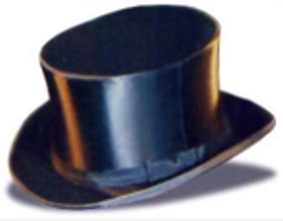
\includegraphics[width=0.8\linewidth]{imagenes/results/caltech/top_hat.png}\\
		{\small (a) Top Hat}
	\end{minipage}\hfill
	\begin{minipage}[t]{0.23\linewidth}
		\centering
		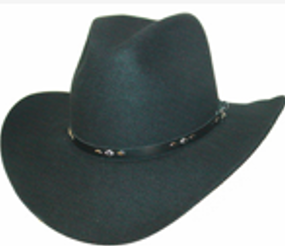
\includegraphics[width=0.8\linewidth]{imagenes/results/caltech/cowboy_hat.png}\\
		{\small (b) Cowboy Hat}
	\end{minipage}\hfill
	\begin{minipage}[t]{0.23\linewidth}
		\centering
		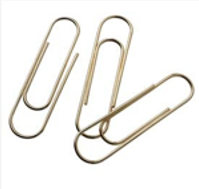
\includegraphics[width=0.8\linewidth]{imagenes/results/caltech/paperclip.png}\\
		{\small (c) Paperclip}
	\end{minipage}\hfill
	\begin{minipage}[t]{0.23\linewidth}
		\centering
		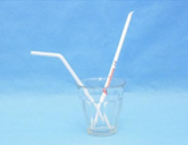
\includegraphics[width=0.8\linewidth]{imagenes/results/caltech/drinking_straw.png}\\
		{\small (d) Drinking Straw}
	\end{minipage}
	
	\vspace{0.4cm}
	
	% --- Row 2 (3 items balanced in the center) ---
	\hfill
	\begin{minipage}[t]{0.23\linewidth}
		\centering
		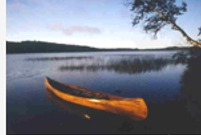
\includegraphics[width=0.8\linewidth]{imagenes/results/caltech/cannoe.png}\\
		{\small (e) Canoe}
	\end{minipage}\hfill
	\begin{minipage}[t]{0.23\linewidth}
		\centering
		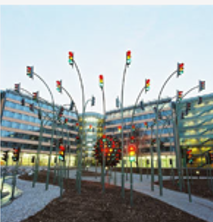
\includegraphics[width=0.8\linewidth]{imagenes/results/caltech/traffic_light.png}\\
		{\small (f) Traffic Light}
	\end{minipage}\hfill
	\begin{minipage}[t]{0.23\linewidth}
		\centering
		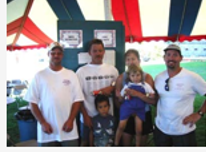
\includegraphics[width=0.8\linewidth]{imagenes/results/caltech/people.png}\\
		{\small (g) People}
	\end{minipage}\hfill\null
	
	\caption{Representative visual entities comprising the minimum separability boundary on the Split Caltech-256 stream mapped to the tracking trends outlined in Table~\ref{tab:worst_diag} and Table~\ref{tab:worst_full}.}
	\label{fig:worst_repr_caltech}
\end{figure}

This qualitative visual inspection confirms the reasoning behind the statistical proximity metrics recorded in our diagnostic tables. Categories such as \textit{boy} and \textit{girl} (Figure~\ref{fig:worst_repr_cifar}a--b), captured at the limited $32\times32$ pixel resolution of Split CIFAR-100, share nearly identical facial structures, skin tone distributions, and foreground composition. Similarly, the overlap between \textit{cloud} and \textit{sea} (Figure~\ref{fig:worst_repr_cifar}e--f) is driven by very similar global color palettes and low-frequency texture statistics, where the boundary between a cloudy sky and an ocean horizon becomes visually continuous. Given these strong semantic and stylistic similarities, it is expected from a generative perspective that their respective class-conditional feature distributions end up in near-coincident regions of the embedding space. The resulting cross-class confusion is therefore not caused by parameter degradation or catastrophic forgetting, but is a natural consequence of modeling independent probability densities over visual representations that are genuinely ambiguous.

\subsection{Synthesis of Inter-Class Confusion and Structural Bounds}
\label{sec:an:confusion}

The pairwise relationships extracted from the distributions once every class has been added (Tables~\ref{tab:worst_diag} and~\ref{tab:worst_full}) give a localized explanation for the separability trends seen across the benchmarks. The framework itself is not breaking down; the residual classification error concentrates in a small tail of highly confusable class pairs, and that tail is what shows where the representation's semantic boundaries actually sit.

This localized failure breaks down into three patterns:
\begin{itemize}
	\item \textbf{Semantic and Visual Near-Synonyms:} The most notable confusion comes from pairs that share basic silhouette, texture, or composition under DINOv2's representation. Cases such as \textit{boy}$\leftrightarrow$\textit{girl} ($D_B = 3.45$, $d_E = 0.145$), \textit{bow\_tie}$\leftrightarrow$\textit{scarf} ($D_B = 16.57$), and \textit{top-hat}$\leftrightarrow$\textit{cowboy-hat} ($D_B = 29.75$) show co-located distributions, where high-frequency discriminative features are largely absent from frozen, general-purpose embeddings.
	\item \textbf{Contextual and Manifold Sinks:} Proximity in the embedding space often comes from shared background or composition rather than category membership. This is shown by the overlap of \textit{cloud}$\leftrightarrow$\textit{sea} ($D_B = 30.54$) through matching color palettes, and by broad categories like \textit{people} acting as confusion sinks for unrelated objects (\textit{canoe}, \textit{drinking-straw}) that happen to be photographed with human subjects in frame.
	\item \textbf{The Mechanics of Apparent Forgetting:} This pairwise crowding is what actually explains the modest rise in forgetting recorded throughout the stream. Class-conditional models are estimated independently and frozen, so the representations themselves do not degrade over time. Apparent forgetting comes strictly from the growth of the label space, which raises the chance of inserting a new category close to one already learned.
\end{itemize}

This also shows the limits of downstream parametric adaptation. Upgrading the modeling architecture from a Diagonal to a Full covariance matrix captures useful correlational structure (recovering \textit{boy} from $50.0\,\%$ to $58.0\,\%$ recall), but it cannot fully separate distributions whose means are nearly the same ($d_E \to 0$). Resolving that remaining overlap is a task for representation alignment at the backbone level. To see how much the whole class-incremental pipeline depends on these native feature distributions, the next section evaluates the sensitivity of the Gaussian framework to the choice of the upstream feature extractor itself.

\section{Sensitivity to the Choice of Backbone}
\label{sec:backbone_results}
\label{sec:method:backbones}

DINOv2~\cite{oquab2024dinov} is the default backbone for the Gaussian-based classifiers in this thesis, chosen for its self-supervised training and the close-to-Gaussian, well-conditioned class-conditional distributions shown in Section~\ref{sec:method:gaussianity_main}. The framework itself does not depend on this particular choice: any frozen encoder that produces fixed-dimensional embeddings can plug into the downstream Gaussian classifier unchanged. To see how much the framework actually depends on the backbone, we re-run Diag-Cov, Full-Cov, and MOG4-Shared using two supervised Vision Transformers from the \texttt{timm} library~\cite{rw2019timm}, \textbf{ViT-base/16} (ViT-b, $d=768$) and \textbf{ViT-medium/16} (ViT-m, $d=512$), both pre-trained on ImageNet-21k~\cite{imagenet21k}, keeping the covariance estimation, hyperparameters, and evaluation protocol identical across backbones.

Table~\ref{tab:multi_backbone_results} reports this comparison across the three benchmarks, for the two best closed-form estimators plus MOG4-Shared, evaluated with three vision backbones: DINOv2-B/14~\cite{oquab2024dinov} (the default used throughout this thesis), ViT-B/16, and ViT-Medium (ViT-M/16).

\begin{table}[htb]
	\centering
	\caption{Impact of backbone architecture on Diag-Cov, Full-Cov, and MOG4-Shared across three benchmarks.}
	\label{tab:multi_backbone_results}
	\begin{adjustbox}{width=0.9\columnwidth, center}
		\small
		\setlength{\tabcolsep}{3.5pt}
		\begin{tabular}{l|c|cc|cc|cc}
			\hline
			\multirow{2}{*}{\textbf{Method}} & \multirow{2}{*}{\textbf{Backbone}} & \multicolumn{2}{c|}{\textbf{CIFAR-100}} & \multicolumn{2}{c|}{\textbf{ImageNet-R}} & \multicolumn{2}{c}{\textbf{Caltech-256}} \\
			\cline{3-8}
			& & $A_{10} (\uparrow)$ & $F_{10} (\downarrow)$ & $A_{10} (\uparrow)$ & $F_{10} (\downarrow)$ & $A_{10} (\uparrow)$ & $F_{10} (\downarrow)$ \\
			\hline
			\multirow{3}{*}{Diag-Cov}
			& DINOv2-B/14 & $86.07 \pm 0.00$ & $4.30 \pm 0.12$ & $\mathbf{77.12 \pm 0.00}$ & $7.44 \pm 0.17$ & $90.06 \pm 0.00$ & $1.69 \pm 0.36$ \\
			& ViT-M/16    & $81.41 \pm 0.00$ & $5.28 \pm 0.13$ & $66.11 \pm 0.00$ & $\mathbf{4.79 \pm 0.14}$ & $\mathbf{91.41 \pm 0.00}$ & $\mathbf{1.63 \pm 0.12}$ \\
			& ViT-B/16    & $81.03 \pm 0.00$ & $4.57 \pm 0.41$ & $43.08 \pm 0.00$ & $6.41 \pm 0.19$ & $87.72 \pm 0.00$ & $1.74 \pm 0.50$ \\
			\hline
			\multirow{3}{*}{Full-Cov}
			& DINOv2-B/14 & $\mathbf{88.38 \pm 0.00}$ & $\mathbf{4.12 \pm 0.00}$ & $74.71 \pm 0.00$ & $5.16 \pm 0.02$ & $\mathbf{94.93 \pm 0.01}$ & $1.74 \pm 0.05$ \\
			& ViT-M/16    & $82.42 \pm 0.01$ & $5.25 \pm 0.01$ & $66.44 \pm 0.01$ & $5.21 \pm 0.14$ & $92.14 \pm 0.00$ & $2.53 \pm 0.12$ \\
			& ViT-B/16    & $82.40 \pm 0.00$ & $5.27 \pm 0.36$ & $46.23 \pm 0.00$ & $6.34 \pm 0.12$ & $87.13 \pm 0.00$ & $1.92 \pm 0.80$ \\
			\hline
			\multirow{3}{*}{MOG4-Shared}
			& DINOv2-B/14 & $\mathbf{88.98 \pm 0.00}$ & $4.03 \pm 0.09$ & $\mathbf{80.19 \pm 0.00}$ & $\mathbf{4.44 \pm 0.12}$ & $94.61 \pm 0.00$ & $1.88 \pm 0.09$ \\
			& ViT-M/16    & $85.57 \pm 0.00$ & $5.04 \pm 0.09$ & $70.03 \pm 0.00$ & $3.67 \pm 0.10$ & $93.93 \pm 0.00$ & $2.27 \pm 0.08$ \\
			& ViT-B/16    & $84.59 \pm 0.00$ & $4.72 \pm 0.06$ & $47.20 \pm 0.00$ & $4.64 \pm 0.13$ & $89.49 \pm 0.00$ & $2.01 \pm 0.140$ \\
			\hline
		\end{tabular}
	\end{adjustbox}
\end{table}

\subsection{Interpreting the Backbone Comparison}
\label{sec:an:backbone}

Table~\ref{tab:multi_backbone_results} shows that backbone choice is the single largest factor for the framework. DINOv2 beats the supervised alternatives by 5--35 accuracy points on CIFAR-100 and ImageNet-R; ViT-B/16 in particular drops to 43--47\,\% on ImageNet-R. Caltech-256 is the exception: all three backbones land within about four accuracy points of each other, since its categories are already easy to separate visually, which moves the bottleneck from the encoder to the downstream classifier and makes the choice of backbone matter less.

MOG4-Shared follows the same pattern as Diag-Cov and Full-Cov, and it is the best performer with every backbone tested. With DINOv2 it reaches $88.98\%$/$80.19\%$/$94.61\%$ on CIFAR-100/ImageNet-R/Caltech-256, at or above the best of the other two estimators on every benchmark. Moving to ViT-M/16 or ViT-B/16 costs it roughly the same, proportionally, as it costs Diag-Cov and Full-Cov, so a weaker backbone drags down every estimator by a similar margin rather than singling one out. In other words, DINOv2 is not just the better choice for this particular estimator; it is the better choice regardless of which covariance estimator sits on top of it.

Beyond the covariance estimators and backbones evaluated above, the next section turns to the statistical structure of the embedding space itself, beginning with its spectral geometry.

\section{Spectral Analysis of the DINOv2 Embedding Space}
\label{sec:spectral_analysis}
\phantomsection\label{sec:pca_results}
\phantomsection\label{sec:an:embedding}

Chapter~\ref{ch:gaussian_space} introduced spectral decay: how quickly the eigenvalues of the feature covariance shrink tells us whether an embedding is genuinely high-dimensional or effectively lives in a much smaller subspace. Here we apply that idea to the DINOv2 embeddings used throughout this chapter, computing the empirical spectrum of the $\ell_2$-normalised features, pooled across each benchmark's training split.

\begin{figure}[htbp]
	\centering
	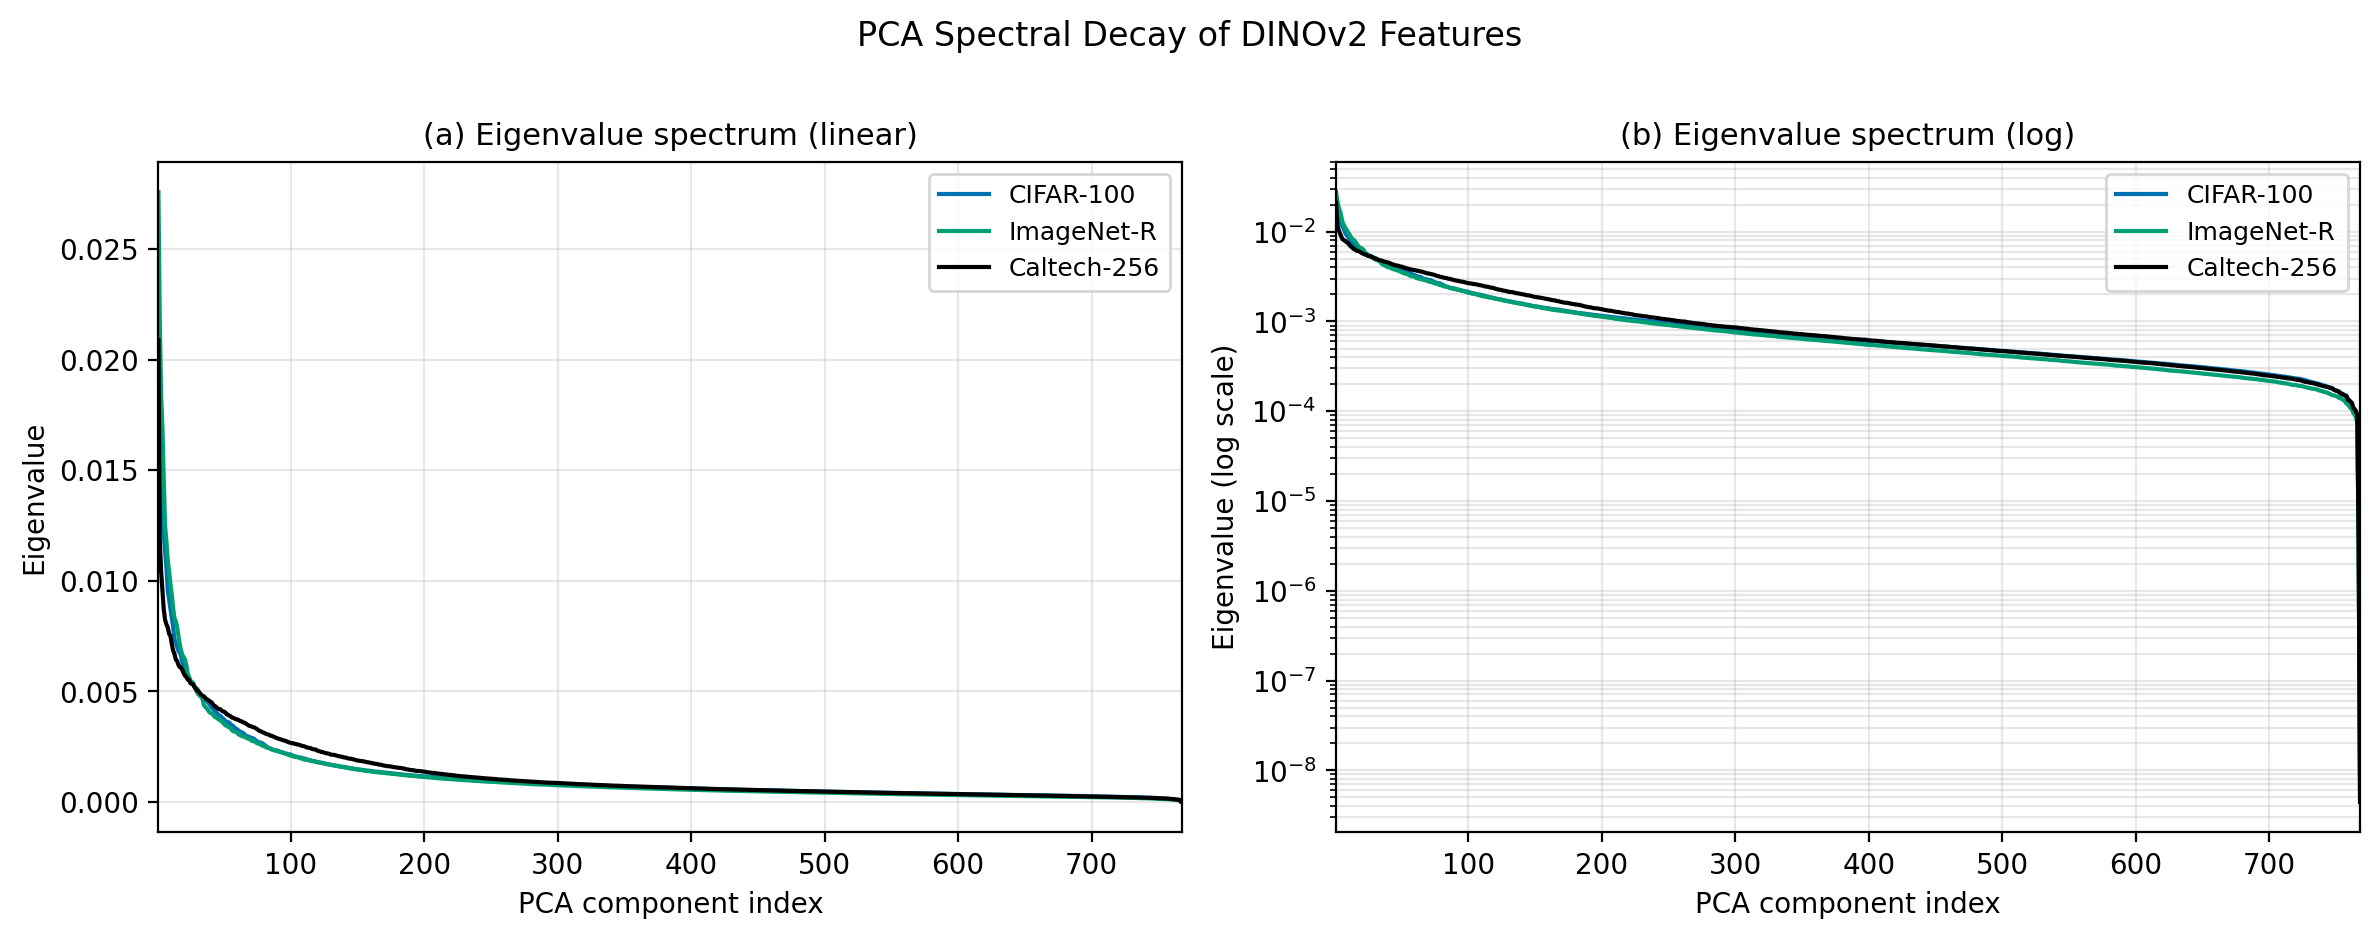
\includegraphics[width=0.97\linewidth]{imagenes/results/pca_eigenvalues.png}
	\caption{PCA spectral decay of the $\ell_2$-normalised DINOv2 features. \textbf{(a)} Individual \% variance explained per component: steep decay over the first $\sim\!50$ components, near-zero contribution thereafter. \textbf{(b)} Cumulative \% variance explained: dashed reference lines mark 50, 80, 90 and 95\,\%; annotated $n$ values show how many components suffice to reach 90\,\% on each dataset. Despite the $d=768$ embedding space, $90\,\%$ of the variance is captured by fewer than 130 components on every benchmark.}
	\label{fig:pca_eigenvalues}
\end{figure}

One notable feature of this spectrum is how similar it looks across very different image distributions. As shown in Figure~\ref{fig:pca_eigenvalues}, the decay curves for Split CIFAR-100, Split ImageNet-R, and Split Caltech-256 overlap almost exactly, so DINOv2 spreads variance across its coordinates in roughly the same way whether it is processing low-resolution natural images, artistic renditions, or high-resolution object photography. Because of this, there is no need to tune the dimensionality separately for each dataset, and the same probabilistic modelling layer can be used across all of them.

\subsection{Spectral Properties of the Foundation Embeddings}
\label{sec:an:spectrum}

The spectrum in Figure~\ref{fig:pca_eigenvalues} shows three consistent patterns across the DINOv2 feature space.

First, all three benchmarks allocate variance in a similar multi-stage way. The first principal component accounts for roughly 8\%--10\% of the total variance, followed by a sharp decay over the first $\sim\!50$ dimensions that together capture 36\%--40\% of the global variance. Beyond that point, the spectrum flattens into a long tail that decays slowly across the remaining 700+ coordinates.

Second, there is no abrupt cutoff in the spectrum. Most of the discriminative signal sits in a moderate-dimensional subspace, but it is not confined to it entirely: some real variability is spread across the whole ambient space. This is why we use a full, high-dimensional ($d=768$) generative model instead of a truncated, PCA-reduced one by default.

Third, and independently of this global spectrum, the effective rank of any per-class empirical covariance matrix is bounded above by $n_c - 1$, since at most $n_c - 1$ directions can be populated from $n_c$ centred observations. When $n_c < d$, this bound alone forces rank deficiency, and it is the root cause of the numerical instability we saw earlier in unconstrained full-covariance estimation. The next subsection tests directly whether the concentration of variance shown here can be used to work around it.

\subsection{Empirical Validation via Subspace Compression Tracking}
\label{sec:pca_cl_results}

If most of the variance really does sit in a moderate-dimensional subspace, compressing the features before classification should recover most of the rank deficiency problem discussed above, at the cost of throwing away only the low-variance tail. To test this, we project the DINOv2 embeddings down to $d=64$ and $d=256$ dimensions and re-run the class-incremental classifiers on the compressed features. Table~\ref{tab:pca_accuracy} reports the average accuracy once every class has been added, across three independent class-ordering runs. As with the uncompressed results, the class-conditional statistics come from a fixed training partition, so the standard deviation is zero across all cells: which order the classes arrive in does not change where the estimator converges.

\begin{table}[htbp]
	\centering
	\caption{Final average accuracy (\%) of the Gaussian continual-learning classifier after projecting DINOv2 embeddings to $d\!\in\!\{64,\,256\}$ dimensions via PCA. \emph{Diag}: diagonal covariance; \emph{Full}: full covariance with adaptive ridge regularisation. Higher is better.}
	\label{tab:pca_accuracy}
	\small
	\setlength{\tabcolsep}{5pt}
	\begin{tabular}{l|ccc|ccc}
		\toprule
		& \multicolumn{3}{c|}{\textbf{PCA $d=64$}} & \multicolumn{3}{c}{\textbf{PCA $d=256$}} \\
		\textbf{Benchmark} & Diag & Full & MOG4-Shared & Diag & Full & MOG4-Shared \\
		\midrule
		CIFAR-100      & 78.48 & \textbf{83.05} & 82.24 & 85.22 & 82.29 & \textbf{88.16} \\
		ImageNet-R     & 64.04 & 49.65 & \textbf{66.84} & 71.79 & 61.25 & \textbf{77.06} \\
		Caltech-256    & 87.20 & 43.40 & \textbf{90.58} & 90.01 & 91.09 & \textbf{94.42} \\
		\bottomrule
	\end{tabular}
\end{table}

The behavior across dimensionalities maps directly onto the shape of the spectrum described above. Scaling the PCA dimensionality from $d=64$ to $d=256$ lifts Diag-Cov's accuracy on every benchmark ($+6.7$\,pp on Split CIFAR-100, $+7.8$\,pp on Split ImageNet-R, $+2.8$\,pp on Split Caltech-256), confirming that although fewer than 130 components already capture 90\% of the variance, the remaining low-variance tail still holds fine-grained information that helps resolve close class boundaries.

MOG4-Shared benefits from this compression even more than Diag-Cov does. At $d=256$ it is the best of the three methods on every benchmark ($88.16\%$ on CIFAR-100, $77.06\%$ on ImageNet-R, $94.42\%$ on Caltech-256), and at $d=64$ it already leads on ImageNet-R and Caltech-256, trailing Full-Cov by less than a point on CIFAR-100 ($82.24\%$ vs. $83.05\%$). This follows from the same mechanism discussed in Section~\ref{sec:an:homoscedasticity}: MOG4-Shared estimates a single covariance from the pooled residuals of every active class, so compressing the features still leaves it with plenty of data to estimate that one covariance well. Full-Cov, by contrast, has to fit a separate covariance per class from a much smaller sample, which is exactly what causes it to struggle under compression, as the next subsection shows in more detail.

\subsection{Covariance Parameterisations and Subspace Interplay}
\label{sec:pca_covariance_interplay}

The gap between Diag-Cov and Full-Cov shows two sides of the same regularisation problem under data scarcity. On Split CIFAR-100 at $d=64$, compression actually helps Full-Cov: the sample budget ($n_c=400$) comfortably exceeds the projection dimension, so it can exploit stable off-diagonal correlations and beat Diag-Cov by $+4.6$\,pp. Expanding to $d=256$ reverses this into a $-2.9$\,pp deficit, since even within the leading part of the spectrum, the number of free parameters starts to outpace how much data is available.

This same effect causes a sharp drop for Full-Cov on the sample-starved streams of ImageNet-R ($n_c=40$) and Caltech-256 ($n_c=64$) under heavy compression. At $d=64$, Full-Cov's unconstrained covariance becomes rank-deficient, losing $14.4$\,pp on ImageNet-R and $43.8$\,pp on Caltech-256 relative to Diag-Cov. These gaps narrow as dimensionality expands to $d=256$, where Full-Cov eventually reaches the peak accuracy on Caltech-256 ($91.09\%$), but the pattern still shows that a linear dimensionality reduction can distort per-class correlations whenever the sample budget stays close to the projection size. MOG4-Shared avoids this failure mode altogether, for the reason given above: it never has to estimate an independent covariance from a small, per-class sample in the first place.

\section{Validating the DINOv2 Gaussianity Assumption}
\label{sec:gaussianity_results}

Chapter~\ref{ch:gaussian_space} checked Gaussianity at two levels: per-dimension, whether each coordinate on its own looks Gaussian, and per-class, whether the full, high-dimensional feature vector of each class does. Here we apply both checks to the actual DINOv2 embeddings used throughout this thesis, using the training split of each benchmark.

\subsection{Per-Dimension Gaussianity}
\label{sec:uv_gaussianity}

\textbf{Shape moments.}
We compute the sample skewness and excess kurtosis defined in Chapter~\ref{ch:gaussian_space} for every (class $c$, dimension $j$) pair.

\begin{table}[htb]
    \centering
    \caption{Per-dimension Gaussianity statistics over all $(C \times d)$ (class, dimension) pairs per dataset ($d=768$). $|\!\mathrm{Skew}|_\mu$ and $|\!\mathrm{Kurt}|_\mu$ are mean absolute values; $\mathbb{P}[\cdot]$ is the fraction of pairs satisfying each cut-off.}
    \label{tab:gaussianity_stats}
    \scriptsize
    \setlength{\tabcolsep}{4pt}
    \begin{tabular}{lcc cc cc}
        \toprule
        \textbf{Dataset} & \textbf{pairs} & $|\!\mathrm{Skew}|_\mu$ & $\mathrm{Skew}_\sigma$ & $\mathbb{P}[|\mathrm{Skew}|{<}0.5]$ & $|\!\mathrm{Kurt}|_\mu$ & $\mathbb{P}[|\mathrm{Kurt}|{<}1]$ \\
        \midrule
        CIFAR-100   & 76,800  & $0.181$ & $0.236$ & $0.961$ & $0.264$ & $0.982$ \\
        ImageNet-R  & 153,600 & $0.269$ & $0.348$ & $0.859$ & $0.432$ & $0.924$ \\
        Caltech-256 & 192,000 & $0.360$ & $0.472$ & $0.747$ & $0.659$ & $0.822$ \\
        \bottomrule
    \end{tabular}
\end{table}

Table~\ref{tab:gaussianity_stats} reports aggregate statistics. Mean skewness is essentially zero on all benchmarks ($|\overline{\mathrm{Skew}}| \le 0.002$). The fraction of pairs satisfying $|\mathrm{Skew}|<0.5$ drops from $96.1\%$ on CIFAR-100 to $74.7\%$ on Caltech-256, reflecting the smaller per-class sample count and greater visual diversity of the latter.

\textbf{D'Agostino--Pearson test.}
We apply the joint hypothesis test defined in Chapter~\ref{ch:gaussian_space}, rejecting $H_0$ at $\alpha=0.05$, and report the fraction of pairs passing in Table~\ref{tab:gaussianity_normaltest}. With $\bar{n}_c \approx 400$, $120$, and $90$ for CIFAR-100, ImageNet-R, and Caltech-256 respectively, the test gets stricter as the sample grows, so even small, harmless departures from normality get flagged on the larger datasets; even so, $70$--$81\%$ of all pairs pass it, and the relaxed criterion from Chapter~\ref{ch:gaussian_space} ($|\mathrm{Skew}|<1$ and $|\mathrm{Kurt}|<1$) is satisfied by $82$--$98\%$.

\begin{table}[htb]
    \centering
    \caption{Per-feature normality tests on the training split (fractions of $(C \times d)$ pairs). \emph{normaltest}: D'Agostino--Pearson $\chi^2_2$ at $\alpha{=}0.05$. \emph{relaxed}: $|\mathrm{Skew}|<1$ and $|\mathrm{Kurt}|<1$ simultaneously.}
    \label{tab:gaussianity_normaltest}
    \scriptsize
    \setlength{\tabcolsep}{6pt}
    \begin{tabular}{lccc}
        \toprule
        \textbf{Dataset} & \textbf{Normaltest (\%)} & \textbf{Relaxed (\%)} & \textbf{Both (\%)} \\
        \midrule
        CIFAR-100   & $70.0$ & $97.8$ & $70.0$ \\
        ImageNet-R  & $80.8$ & $91.6$ & $79.7$ \\
        Caltech-256 & $73.4$ & $82.3$ & $71.3$ \\
        \bottomrule
    \end{tabular}
\end{table}

\textbf{Henze--Zirkler test per dimension.}
\phantomsection\label{sec:uv_hz_gaussianity_results}
As a stricter check, we also apply the univariate Henze--Zirkler (HZ) test defined in Chapter~\ref{ch:gaussian_space} independently to every $(c,j)$ pair, using $d=1$ and the same finite-sample expectation and bandwidth given there.

\begin{table}[htb]
	\centering
	\caption{Summary results from computing the univariate Henze--Zirkler test statistic over all $(C \times d)$ class-dimension pairs on the training split. $\mathbb{E}_{H_0}[T_{\mathrm{HZ}}]$ is the theoretical expectation under perfect normality, as defined in Chapter~\ref{ch:gaussian_space}, evaluated at the per-class sample size $n_c$.}
	\label{tab:gaussianity_hz_univariate}
	\scriptsize
	\setlength{\tabcolsep}{4pt}
	\begin{tabular}{lcc c}
		\toprule
		\textbf{Dataset} & $\tilde{n}_c$ & $\mathbb{E}_{H_0}[T_{\mathrm{HZ}}]$ & $T_{\mathrm{HZ}}$ mean\,$\pm$\,std \\
		\midrule
		CIFAR-100  & 500 & $\approx 0.04$ & $0.00052 \pm 0.00095$ \\
		ImageNet-R  & 137 & $\approx 0.06$ & $0.00134 \pm 0.00210$  \\
		Caltech-256 & 100 & $\approx 0.07$ & $0.00234 \pm 0.00379$  \\
		\bottomrule
	\end{tabular}
\end{table}

Taken together, these three diagnostics agree: the individual coordinates of the foundation feature vectors have symmetric shapes, near-zero skewness, and little excess kurtosis, and the observed HZ scores sit orders of magnitude below their theoretical $H_0$ expectation. Every marginal, taken on its own, looks close to Gaussian.

\subsection{Per-Class Gaussianity}
\label{sec:mv_gaussianity_results}

Per-dimension normality is necessary but not sufficient: a set of coordinates can each look Gaussian on their own while still not being jointly Gaussian, so we now test each class's full $d=768$-dimensional feature vector at once, using the same HZ statistic as before but with $d$ set to the full embedding dimension. As explained in Chapter~\ref{ch:gaussian_space}, this runs into the same problem as everywhere else in this thesis: since $n_c < d$ for every benchmark, the full covariance matrix needed for the standard version of the test cannot be inverted.

We work around this the same way: by using a diagonal version of the covariance, so only the $d$ per-coordinate variances need to be inverted instead of the full matrix. This changes what to expect under $H_0$ as well. In the univariate case above, a Gaussian coordinate gives $T_{\mathrm{HZ}}$ close to $0$; here, because $d$ is large, the same expectation formula pushes the reference value close to $1$ instead. Table~\ref{tab:gaussianity_hz} shows that all three benchmarks concentrate tightly around $T_{\mathrm{HZ}} = 1$, right where a Gaussian class should land under this diagonal test.

\begin{table}[htb]
    \centering
    \caption{Summary results from computing the diagonal HZ test statistic over all classes in the ambient foundation feature space ($d=768$), using all available training samples. Values concentrated near $T_{\mathrm{HZ}} \approx 1.00$ indicate convergence toward empirical multivariate Gaussianity under the feature-independence assumption.}
    \label{tab:gaussianity_hz}
    \scriptsize
    \setlength{\tabcolsep}{4pt}
    \begin{tabular}{lcc c}
        \toprule
        \textbf{Dataset} & $C$ & $T_{\mathrm{HZ}}$ mean\,$\pm$\,std \\
        \midrule
        CIFAR-100   & 100 & $1.0002 \pm 0.0020$  \\
        ImageNet-R  & 200 & $1.0033 \pm 0.0073$ \\
        Caltech-256 & 250 & $1.0016 \pm 0.0089$ \\
        \bottomrule
    \end{tabular}
\end{table}

As already noted in Chapter~\ref{ch:gaussian_space}, restricting this test to a diagonal covariance means it cannot guarantee full, unconstrained multivariate Gaussianity, where every pair of dimensions is allowed to correlate freely. But given how little data is available per class relative to the embedding dimension, this diagonal version is the only one we can actually compute, and it works as a reasonable stand-in for the stronger, unconstrained test. The consistent convergence to $T_{\mathrm{HZ}} \approx 1.00$ across all three benchmarks is what supports using independent-feature probabilistic classifiers on this embedding space.

\subsection{Empirical Validation of the Gaussian Assumption}
\label{sec:an:gauss}

The Gaussianity tests above confirm that the per-coordinate normality assumption is well supported across all three benchmarks: 96.1\,\% of CIFAR-100 coordinates, 85.9\,\% of ImageNet-R, and 74.7\,\% of Caltech-256 satisfy the informal symmetry cut-off $|\text{Skew}|<0.5$. The key distinction between the two covariance estimators follows directly from the $n_c < d$ regime. The \textbf{Diag-Cov} model estimates only $d$ parameters per class and is therefore always well-conditioned; its squared Mahalanobis distances are broadly distributed near the theoretical $\chi^2_{d=768}$ mode, with dispersion growing from CIFAR-100 to Caltech-256 in line with the heavy-tail ordering of Table~\ref{tab:gaussianity_stats}. The \textbf{Full-Cov} model, by contrast, requires estimating a $d\times d$ matrix from $n_c < d$ samples: the resulting covariance is rank-deficient, the eigenvalues outside the spanned subspace collapse to the regularisation floor, and the quadratic form becomes degenerate, producing a sharp spike at $\overline{n_c}-1$ (approximately 498, 168, and 103 on CIFAR-100, ImageNet-R, and Caltech-256 respectively) rather than spreading across the $\chi^2_{768}$ support. This problem comes from the \emph{estimator}, not from the data: the per-coordinate distributions are near-Gaussian, as shown above. Keeping inter-feature correlations while avoiding rank deficiency is still an open challenge; the hybrid variant is one practical way to balance the two.

For \textbf{MOG4-Shared}, the same $n_c < d$ regime explains why it avoids this trade-off in the first place. Because MOG4-Shared estimates a single covariance from the pooled residuals of every active class rather than one covariance per class, it is never forced to invert a $d\times d$ matrix built from a single class's small sample, so it does not run into the rank-deficiency spike that hurts Full-Cov. On top of that, letting each class use up to four centroids means a class does not need its own feature distribution to be a single, unimodal Gaussian to be modelled well: a mixture of a few Gaussians can still fit a class whose marginals depart from normality more than the ones tested here. This is consistent with MOG4-Shared's results throughout this chapter, and it is one more reason it holds up better than either single-covariance model on its own.

\section{Computational Cost and Practical Considerations}
\label{sec:computational_requirements}
\phantomsection\label{sec:an:other}

Weighing accuracy against computational overhead matters for judging whether a lifelong learning framework is actually practical to run. Table~\ref{tab:computational_requirements} reports the inference cost of the Gaussian classification layer, in floating-point operations (FLOPs), needed to score a single pre-embedded test query against every active category once all tasks have been added.

Each covariance parameterisation has a different, predictable cost:
\begin{itemize}
	\item \textbf{Diag-Cov} scores each class with an element-wise weighted squared Euclidean distance, so the cost grows linearly, $\mathcal{O}(C \cdot d)$, where $C$ is the number of active classes and $d=768$ is the feature dimension.
	\item \textbf{Full-Cov} (and, by extension, Hybrid-Cov, whose Mahalanobis term uses the same Cholesky-based whitening) needs a full matrix--vector multiplication per class to account for the off-diagonal correlations, so its cost grows quadratically, $\mathcal{O}(C \cdot d^2)$.
	\item \textbf{MOG4-Shared} scores each class's up-to-four centroids against the one shared covariance, so its cost is $\mathcal{O}(C \cdot \bar{K} \cdot d^2)$, where $\bar{K}$ is the average number of centroids per class. This puts it between Diag-Cov and a hypothetical unshared, full-mixture model in cost, closer to Full-Cov in practice since both are dominated by the same $d^2$ term.
\end{itemize}

\begin{table}[htbp]
	\centering
	\caption{Inference cost of the Gaussian classification stage once every class has been added, in floating-point operations (FLOPs) per query, for the two dominant covariance parameterisations and for MOG4-Shared. For reference, a single forward pass of the DINOv2 ViT-B/14 feature extractor requires approximately $17.56$ GFLOPs.}
	\label{tab:computational_requirements}
	\small
	\setlength{\tabcolsep}{8pt}
	\begin{tabular}{lccc}
		\toprule
		\textbf{Benchmark} & \textbf{Diag-Cov} & \textbf{Full-Cov} & \textbf{MOG4-Shared} \\
		\midrule
		Split CIFAR-100   & $0.46$ MFLOPs & $0.12$ GFLOPs & $0.42$ GFLOPs \\
		Split ImageNet-R  & $0.92$ MFLOPs & $0.24$ GFLOPs & $0.31$ GFLOPs \\
		Split Caltech-256 & $1.15$ MFLOPs & $0.29$ GFLOPs & $0.58$ GFLOPs \\
		\bottomrule
	\end{tabular}
\end{table}

Even the most demanding case in the table, MOG4-Shared on the 250 classes of Split Caltech-256, needs only $0.58$ GFLOPs. That is still under $4\%$ of the cost of a single forward pass through the DINOv2 ViT-B/14 feature extractor itself ($\approx 17.56$ GFLOPs). So while MOG4-Shared is consistently more expensive than Diag-Cov and, on two of the three benchmarks, than Full-Cov too, the frozen backbone is still what dominates the total cost by a wide margin: whichever covariance estimator is used, it adds essentially no overhead at inference time.

\subsection{Computational Footprint and Practical Scalability}
\label{sec:an:compute}

These FLOPs numbers also show up as a real advantage in wall-clock time. On Split CIFAR-100, adding a newly encountered task to our framework takes about two minutes on a standard consumer-grade GPU, and that time is spent entirely on a single, deterministic pass of feature extraction over the raw images, needed to compute the class statistics.

Prompt-tuning methods reported in the literature typically need 10--30 minutes of training per task on similar hardware, since they backpropagate through a pool of learned prompts over several epochs. Because our framework never backpropagates and never needs a rehearsal buffer, it trains 5--15$\times$ faster, which makes it a reasonable option for low-resource or decentralized edge deployment.

\subsection{Limitations and Architectural Open Questions}
\label{sec:an:limits}

The empirical results support the efficiency and calibration of this frozen generative approach, but three limitations are worth being explicit about.

First, the current evaluation pipeline assumes that exact task boundaries are given during training to partition incoming batches. Relaxing this constraint to support task-free continual learning is an important next step, to test whether the decoupled Gaussian updates stay robust when categorical boundaries are blurred or interleaved.

Second, our experimental validation has focused only on visual classification streams. Although the underlying generative mechanics are in principle agnostic to the input modality, running a parallel validation on transformer-encoded text or speech embeddings is needed to check whether the clean Gaussian behavior observed here generalizes to other representation spaces.

Third, an interesting extension is using the well-behaved calibration profiles of our independent configurations for open-world discovery. The strong overconfidence of the Full covariance model makes its predictive metrics unreliable outside its closed label space. However, the well-calibrated Predictive Entropy and Probability Margin of the Diagonal model could be used directly as natural out-of-distribution scores. Investigating this could show whether the framework can flag novel, unlearned semantic categories while keeping its existing performance.

\section{Summary of Findings and Practical Recommendations}
\label{sec:an:summary}

The results in this chapter give an overall picture of the behavior, computational cost, and limitations of closed-form generative classifiers built on frozen foundation embeddings. Taken together, they show that class-incremental learning, in this setting, can be treated as a density-estimation problem in a stationary representation space rather than as a fight against forgetting. The DINOv2 feature manifold agrees well with the marginal normality assumption, passing coordinate-level Gaussianity thresholds for $96\,\%$ of dimensions in Split CIFAR-100, $86\,\%$ in Split ImageNet-R, and $75\,\%$ in Split Caltech-256, and because the representation stays stable as tasks accumulate, the resulting decision boundaries compete with optimization-heavy, prompt-based architectures while staying deterministic, closed-form, and gradient-free.

The classification ceiling of this framework is set mainly by the upstream feature extractor, not by the downstream classifier, as shown by the large performance gaps across different visual backbones in Section~\ref{sec:backbone_results}. Separately from the choice of backbone, classification error is not spread evenly across classes: it concentrates in a small, heavy-tailed set of pairs, under $0.2\,\%$ of all class combinations, where the pairwise Bhattacharyya distance drops below a critical threshold ($D_B < 20$). These are cases of near-synonymous or visually continuous categories, such as \textit{boy}/\textit{girl} at low resolution, or \textit{top-hat}/\textit{cowboy-hat} and \textit{bow\_tie}/\textit{scarf} under domain shift, where second-order statistics alone cannot pull the classes apart. What looks like forgetting in a frozen stream is really just newly introduced categories landing close to ones already learned.

Which covariance estimator to use depends on the sample budget and how homogeneous the incoming stream is. MOG4-Shared is the strongest general-purpose default: pooling one covariance across every active class keeps it numerically stable even when classes come from very different, unevenly sampled sources, and letting each class use up to four centroids still captures visual variety that a single Gaussian would miss, which is why it comes out ahead across every benchmark in Table~\ref{tab:combined_benchmarks}. When the per-class sample size comfortably exceeds the feature dimensionality and the stream is homogeneous, Full-Cov (or Hybrid-Cov under tighter sample budgets) can match or edge it out at a lower computational cost, since it captures off-diagonal correlations directly without needing the shared-covariance machinery. But once the stream mixes sources with very different sample sizes, as in the Joint benchmark, unconstrained per-class covariances break down, and a shared covariance, ideally paired with MOG4-Shared's extra centroids, is the only reliable choice.

These results support the central idea of this thesis: that lifelong learning, in this setting, can be handled as static statistical modelling instead of ongoing parameter optimization. Because the framework only ever computes frozen sufficient statistics, representation drift is not possible by construction, and the practical decision comes down to picking the covariance parameterisation, MOG4-Shared by default, one of the others when its sample budget and computational cost make more sense, that fits the sample density and semantic granularity of the deployment scenario. Chapter~\ref{ch:conclusion} builds on this to discuss the system-level conclusions and the open questions around representation alignment raised here.